\documentclass[a4paper]{article}
\usepackage[francais]{babel}
\usepackage[utf8]{inputenc}
\usepackage[T1]{fontenc}
\usepackage[margin=2.5cm]{geometry}
\usepackage{graphicx}
\usepackage{xspace}
\usepackage{authblk}

\usepackage{xcolor}

\usepackage{hyperref}
\usepackage{diagbox}
\usepackage{listings}

\newcommand{\todo}[1]{\textcolor{red}{\textbf{ToDo} [ \emph{#1} ]}}
\newcommand{\fixme}[1]{\textcolor{purple}{\textbf{FixMe} [ \emph{#1} ]}}
\newcommand{\note}[1]{\textcolor{blue}{\textbf{Note} [ \emph{#1} ]}}

\lstdefinestyle{log}{
  emptylines=1,
  breaklines=true,
  moredelim=**[is][\color{blue}]{@}{.},
  moredelim=**[is][\color{purple}]{!}{.},
  moredelim=**[is][\color{red}]{?}{.},
  moredelim=**[is][\color{orange}]{£}{.},
  xleftmargin=\parindent,
  basicstyle=\scriptsize\sffamily
}


\definecolor{silver}{rgb}{0.7,0.7,0.7}
\definecolor{green}{rgb}{0,0.6,0}

\lstdefinestyle{C}{
  belowcaptionskip=1\baselineskip,
  breaklines=true,
  xleftmargin=\parindent,
  language=C,
  showstringspaces=false,
  basicstyle=\footnotesize\ttfamily,
  keywordstyle=\bfseries\color{green},
  commentstyle=\itshape\color{silver},
  identifierstyle=\color{black},
  stringstyle=\color{red},
  frame=l,
  numbers=left
}

\graphicspath{{logs/}}





\begin{document}

\title{CBD - Practical evaluation}
\author{Florestan de Moor}
\author{Rémi Hutin}
\affil{ENS Rennes, Université de Rennes 1}
\date{24 Mars 2017}

\maketitle


\section*{Introduction}

\todo{ ??? }

\section{Mitigating stragglers/failures in Hadoop}

\paragraph{Question 1.1}

Hadoop system divides the tasks across many nodes, which can have different performances, due for example to hardware reasons.
Thus, one node can slow down the whole system.
To address this issue, a popular approach is speculative tasks.
Tasks which are still running on some nodes are launched again on nodes that have already finished their tasks, thinking that it may be faster.

In this question, we aim to observe this experimentally.
We used 5 nodes in \texttt{paravance} cluster.
We generated with \texttt{randomwriter} a dataset of 20 Go.
We run sort benchmark, with and without speculation.
We then re-do the same, but we also stress all the CPUs of one node during the executions.

The results are available in appendix:

\begin{table}[!ht]
    \centering
\begin{tabular}{|c|c|c|}
    \hline
    \backslashbox{Speculation}{Stress} & Without & With \\
    \hline
                False             &   \figurename~\ref{1.1.specOff.noStress}   &  \figurename~\ref{1.1.specOff.Stress}   \\
    \hline
                True             &   \figurename~\ref{1.1.specOn.noStress}   &  \figurename~\ref{1.1.specOn.Stress}    \\
    \hline
\end{tabular}
\end{table}

The interesting figures are the one with stress.
When speculation is not enabled, we can see that the node stressed (\texttt{paravance-36}) is clearly slowing down the whole execution.
It takes indeed around 1.4 more time than the other nodes to complete its tasks (35 against 25 seconds).
With speculation enabled, we can see that we have killed tasks on this node:
speculative tasks were launched on other nodes and, as they finished earlier, the original tasks were killed.
This is more efficient: the stressed node is only around 1.16 slower than the other nodes (70 against 60 seconds).
Speculative tasks thus seem to improve the performances of the application, as expected.


\paragraph{Question 1.2}

During an execution, a node failure may happen.
The JobTracker receives regular heartbeat signal from the TaskTracker nodes.
If it receives no heartbeat from a node, it waits for a given amount of time before considering it as dead.
This is the expiry time.
When it realize a node is dead, the JobTracker has to resubmit the dead node tasks to other nodes,
and also rerun some previous completed tasks.

In this question, we try to observe this experimentally.
We used 5 nodes in \texttt{parapluie} cluster.
We generated with \texttt{randomwriter} a dataset of 5 Go.
We run executions with two different expiry times : 30 seconds and 60 seconds.
During an execution, we kill the TaskTracker daemon on one node, with two different scenarios:
\begin{itemize}
    \item Before the completion of map tasks
    \item After the completion of map tasks
\end{itemize}

\begin{table}[!ht]
    \centering
\begin{tabular}{|c|c|c|}
    \hline
    \backslashbox{Expiry time}{Completion of map tasks} & Before & After \\
    \hline
                30 seconds             &   \figurename~\ref{1.1.specOff.noStress}   &  \figurename~\ref{1.1.specOff.Stress}   \\
    \hline
                60 seconds             &   \figurename~\ref{1.1.specOn.noStress}   &  \figurename~\ref{1.1.specOn.Stress}    \\
    \hline
\end{tabular}
\end{table}

\todo{ explain 30s 60s no real difference, just takes longer to decide that node is dead, we only have killed after completion of maps: maps and reduce tasks killed, and maps are re-run }



\section{Application specific optimization in Hadoop}

\paragraph{Question 2.1}

During an execution, it is possible to choose when to start the reduce tasks compared to the completed map tasks.
At first, it may seem better to wait for all map tasks to end before running reduce tasks,
but in some situations starting reduce tasks earlier may lead to better performances.
This optimization is application dependent.
Starting reduce tasks earlier spreads out the data transfer over time, which is good if performances are limited by the network.
But on the other hand, reduce tasks occupy slots that may have been used by other tasks.

We used 5 nodes in \texttt{parapluie} cluster.
In this question, we generated with \texttt{randomwriter} a dataset of 5 Go, and with \texttt{randomtextwriter} a dataset of 1 Go.
We denote the reduce start paramater by $p$.
This mean that reduce tasks start when fraction $p$ of map tasks are completed.
We set $p \in \lbrace 0.05, 0.5, 1 \rbrace$.
We run sort benchmark on the 5 Go dataset, and the word count benchmark on the 1 Go dataset.

\begin{table}[!ht]
    \centering
\begin{tabular}{|c|c|c|c|}
    \hline
    \backslashbox{Benchmark}{Reduce slow-start} & 5\% & 50\% & 100\% \\
    \hline
                Sort             &   \figurename~\ref{1.1.specOff.noStress}   &  \figurename~\ref{1.1.specOff.Stress}   & \\
    \hline
                Word count             &   \figurename~\ref{1.1.specOn.noStress}   &  \figurename~\ref{1.1.specOn.Stress}    & \\
    \hline
\end{tabular}
\end{table}

\todo{ explain, word count is more map expensive so slow start should not influence too much, but difference should be visible with sort }

\newpage
\appendix

%% To easily comment if compilation of all figures is
%% too long and is annoying when fixing small things
\section{Question 1.1}

\begin{figure}[!ht]
    \centering
    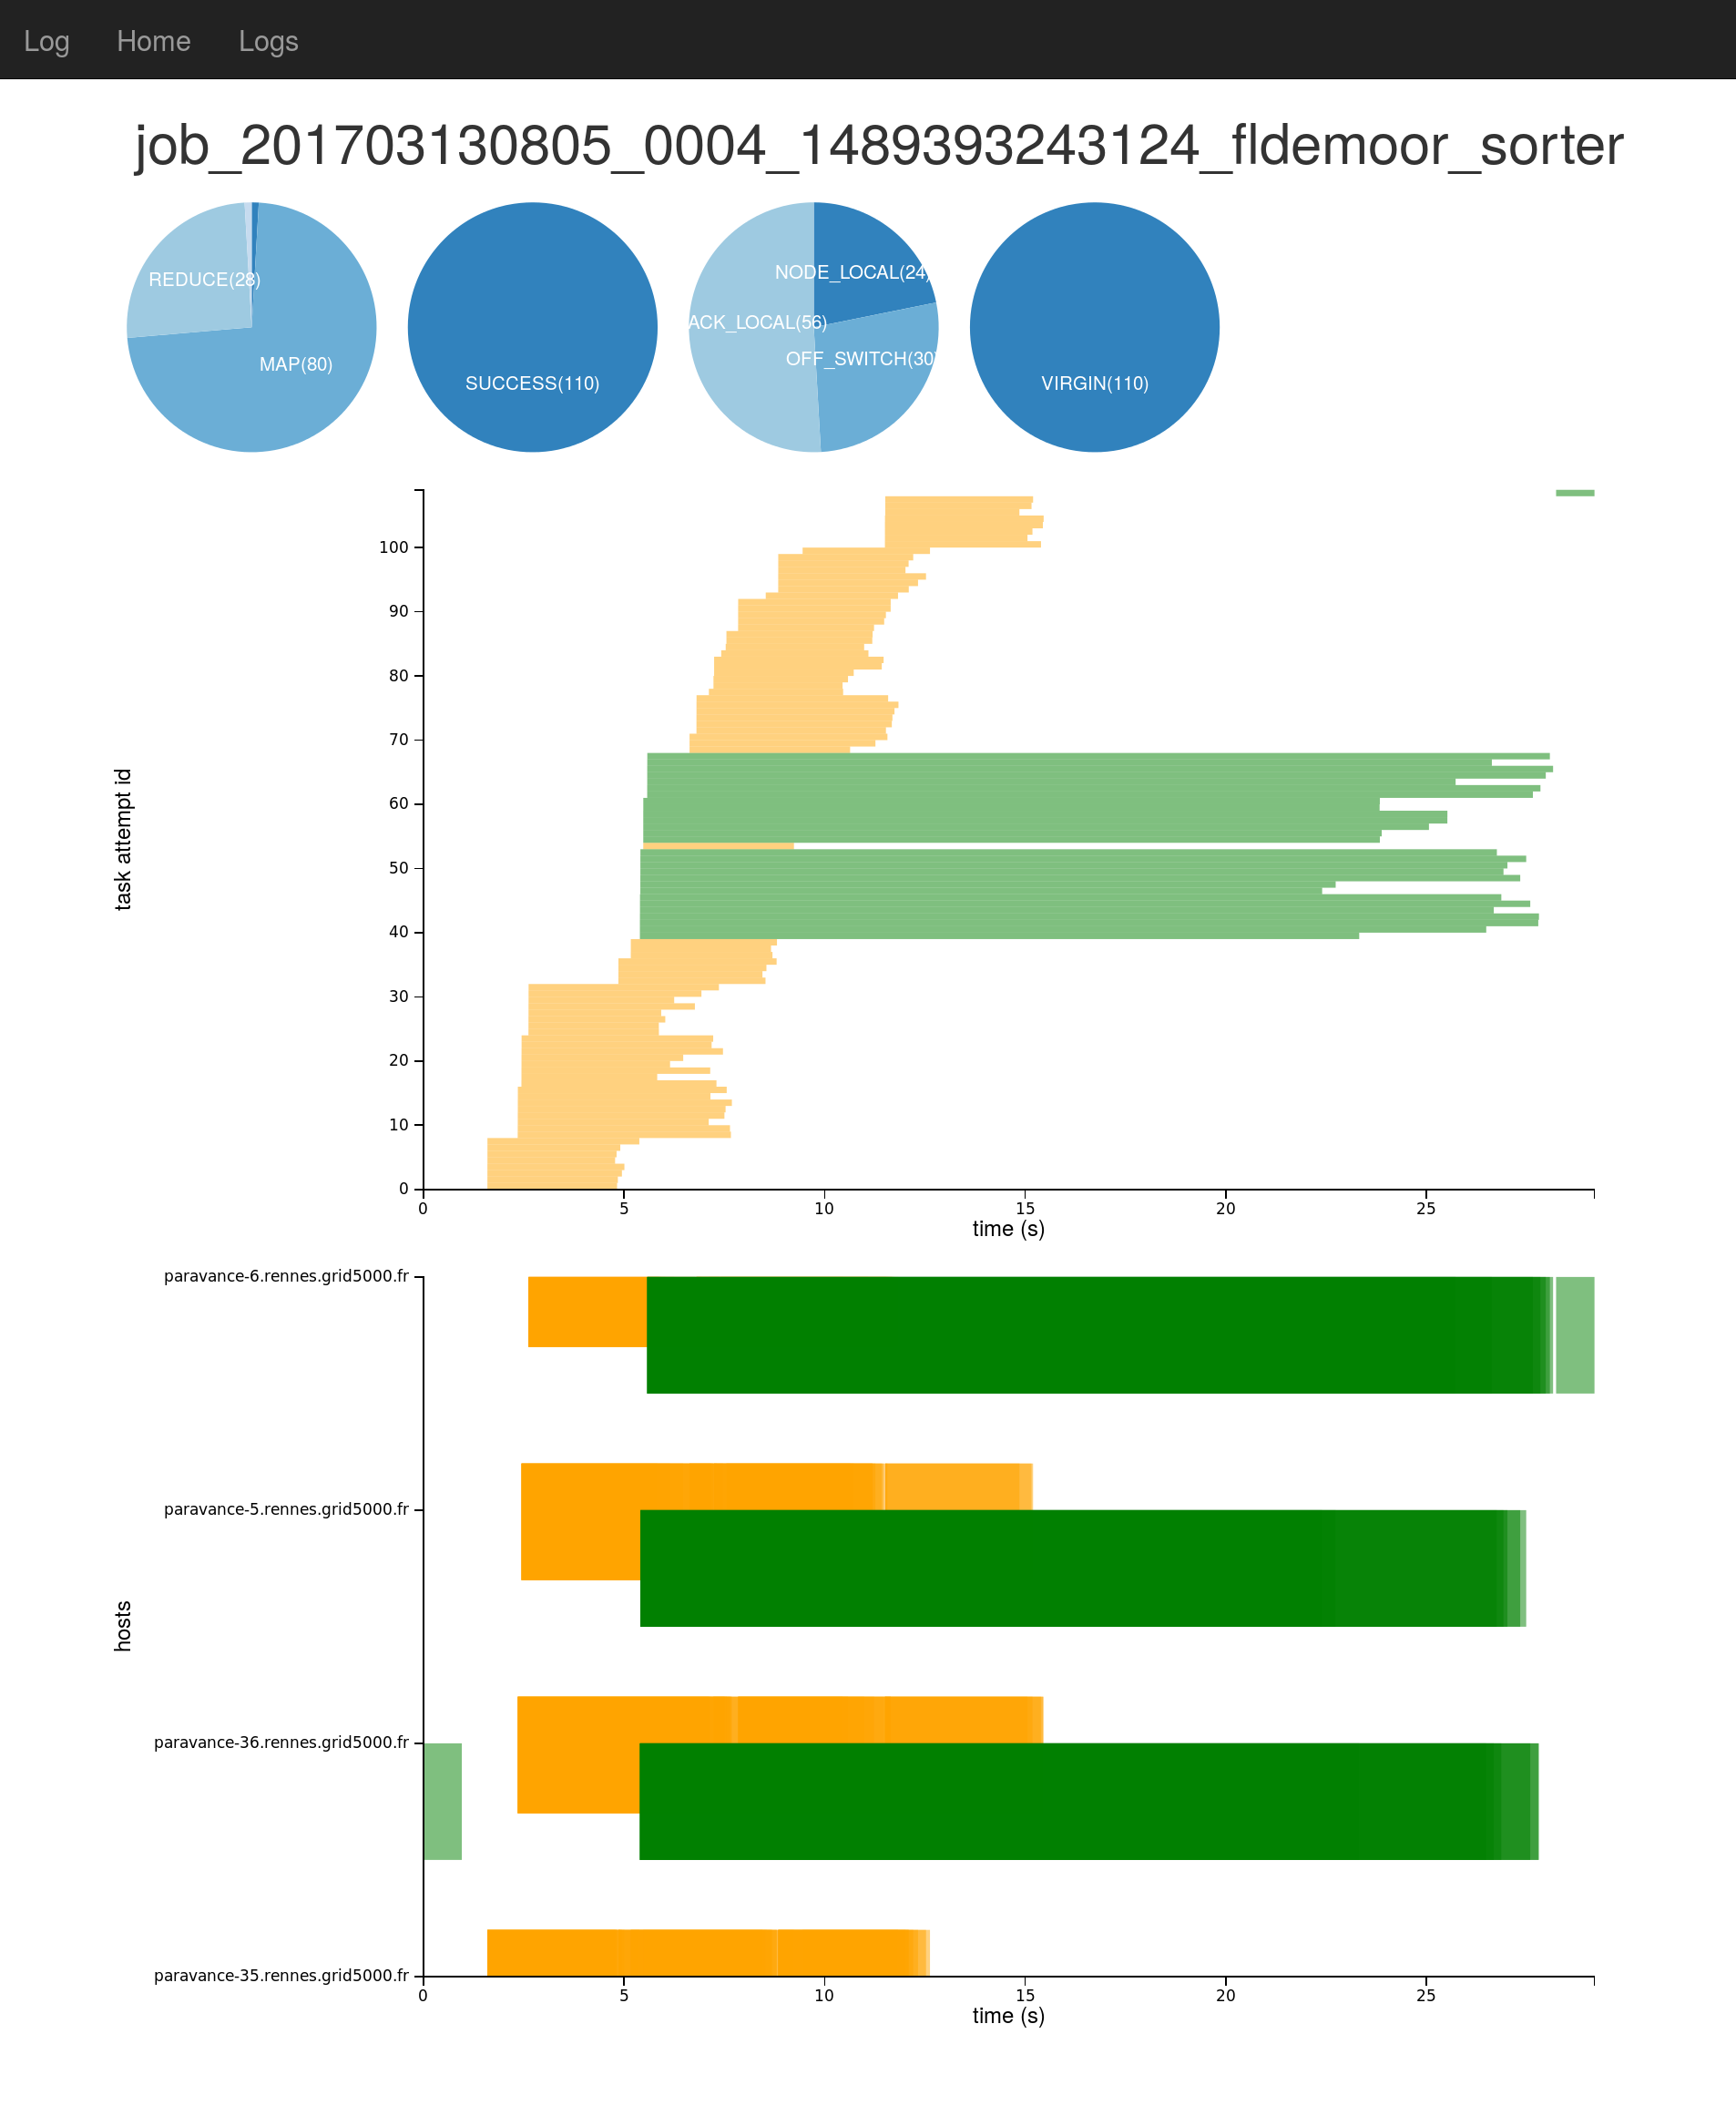
\includegraphics[trim={3.5cm 3.5cm 3.5cm 3.5cm},clip,width=\textwidth]{job_201703130805_0004_1489393243124_fldemoor_sorter_attempts.png}
    \caption{Question 1.1: Without speculation, without stress}
    \label{1.1.specOff.noStress}
\end{figure}
\newpage

\begin{figure}[!ht]
    \centering
    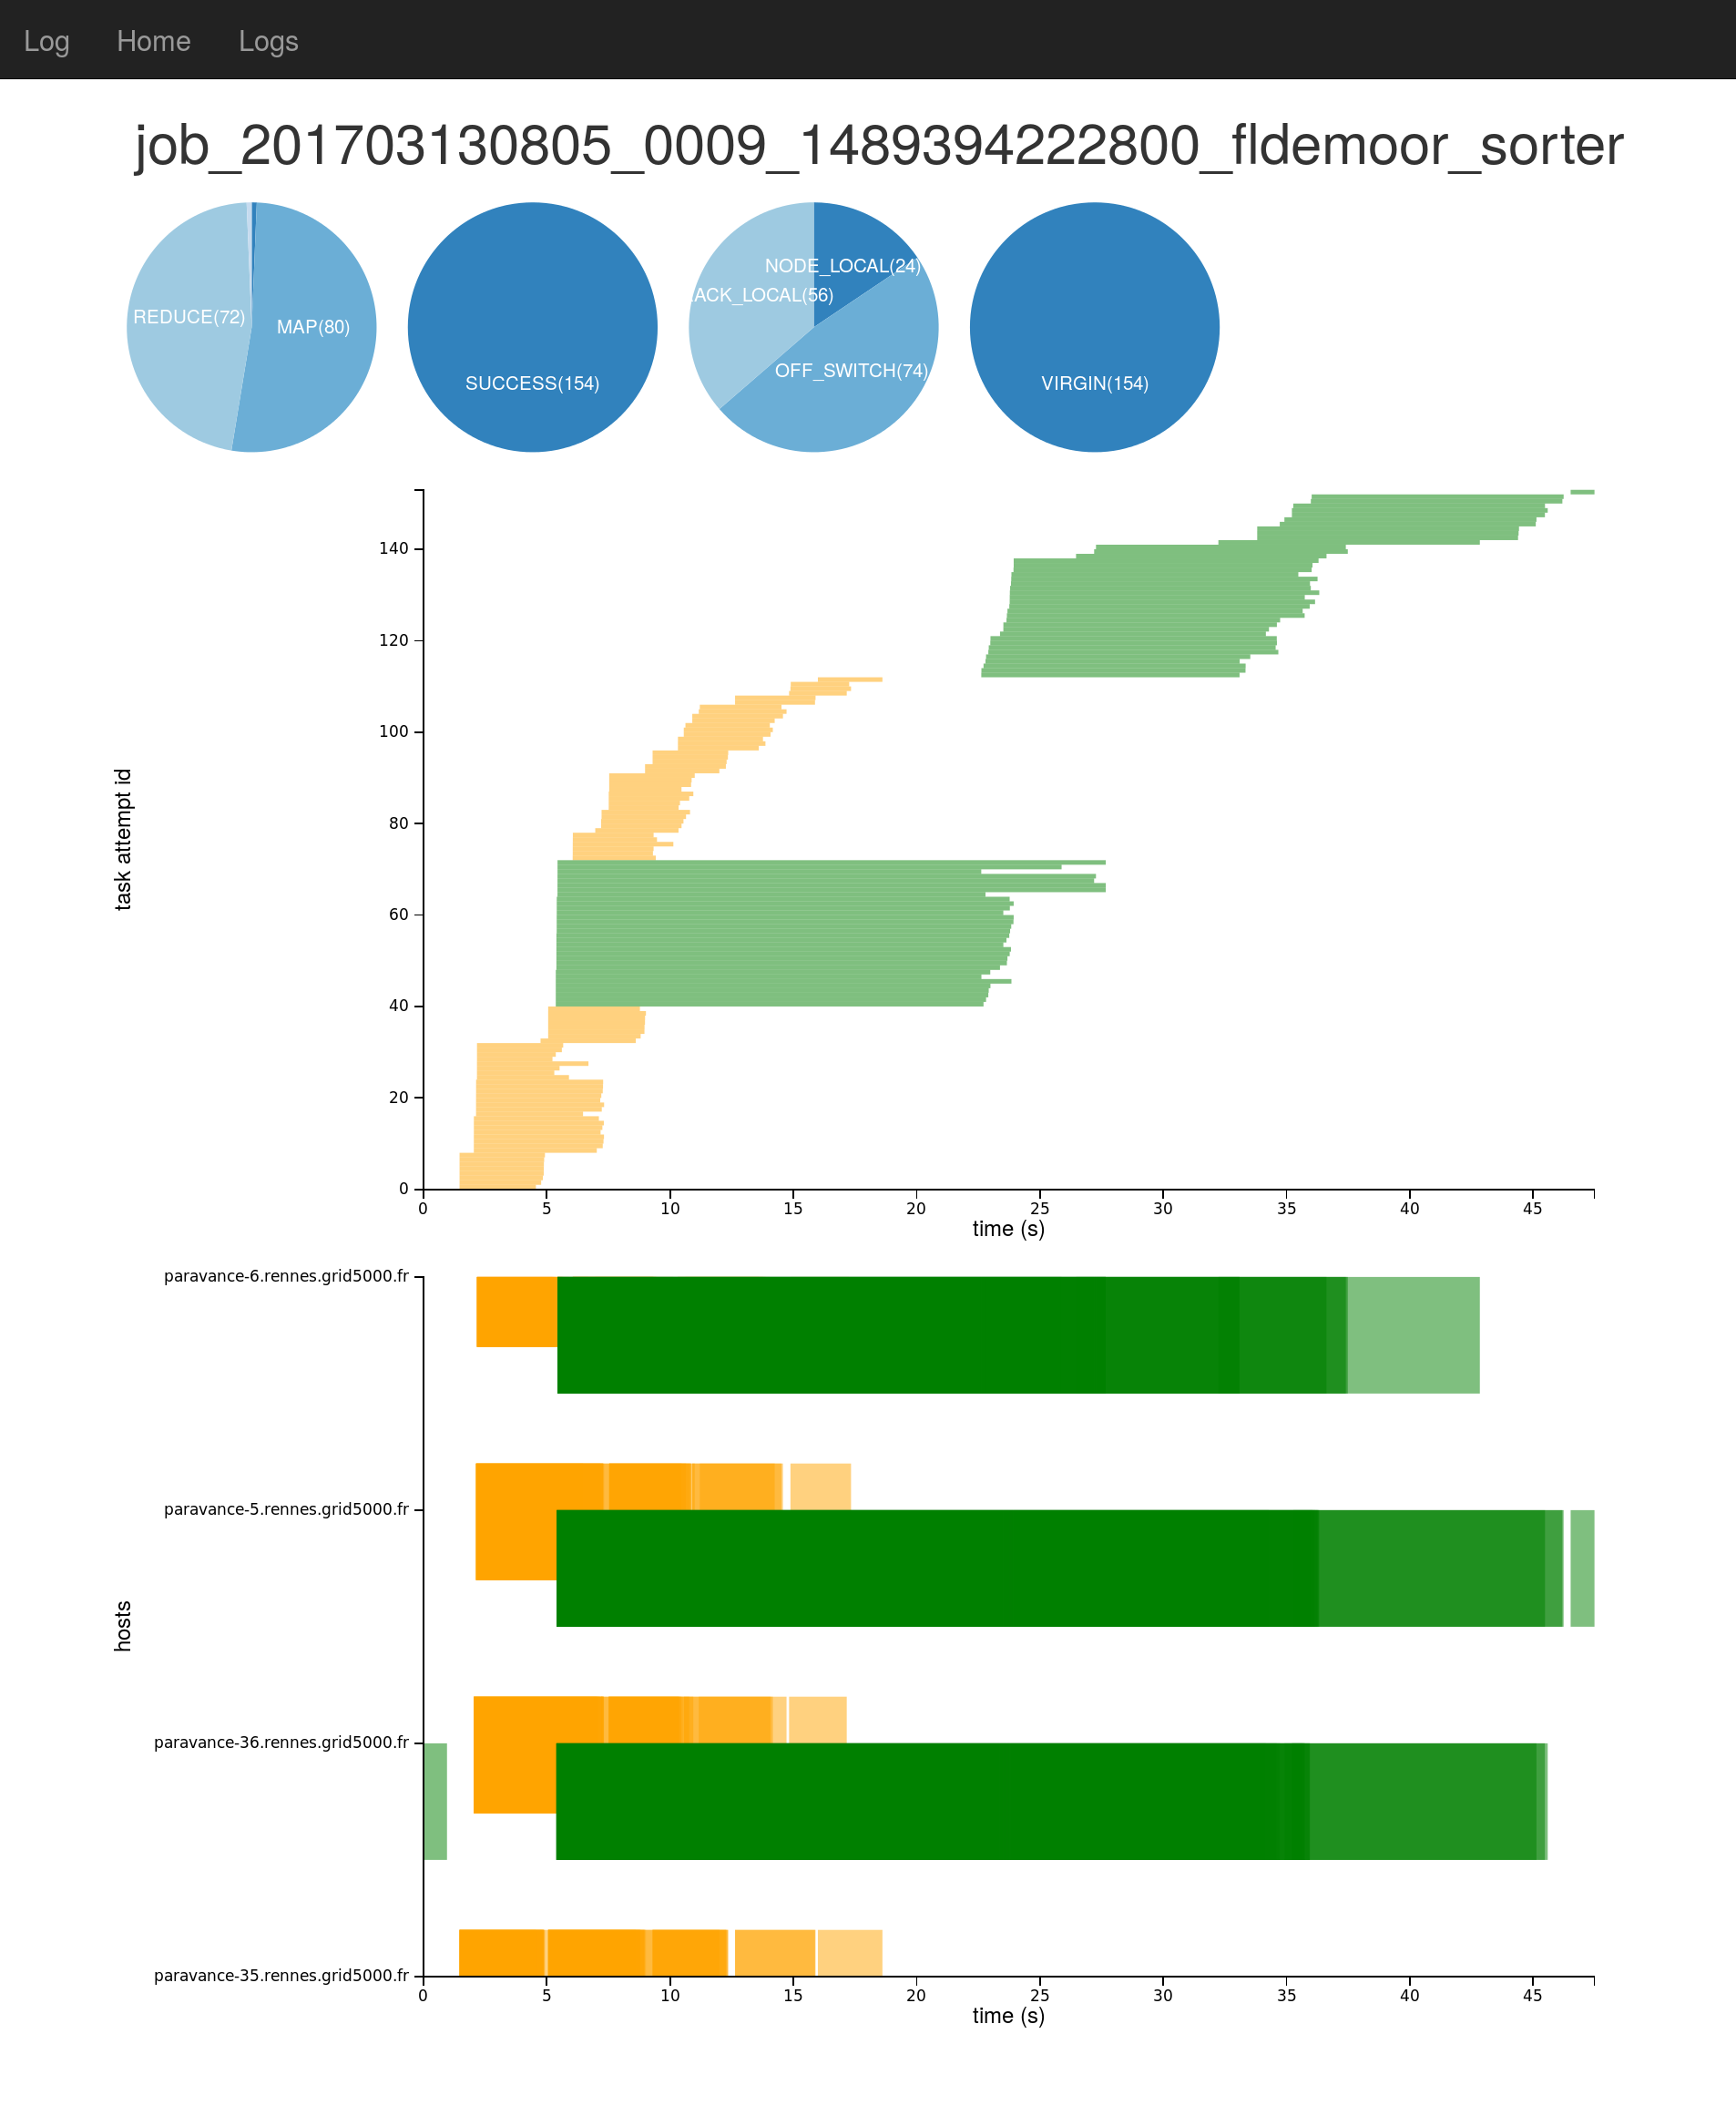
\includegraphics[trim={3.5cm 3.5cm 3.5cm 3.5cm},clip,width=\textwidth]{job_201703130805_0009_1489394222800_fldemoor_sorter_attempts.png}
    \caption{Question 1.1: With speculation, without stress}
    \label{1.1.specOn.noStress}
\end{figure}

\begin{figure}[!ht]
    \centering
    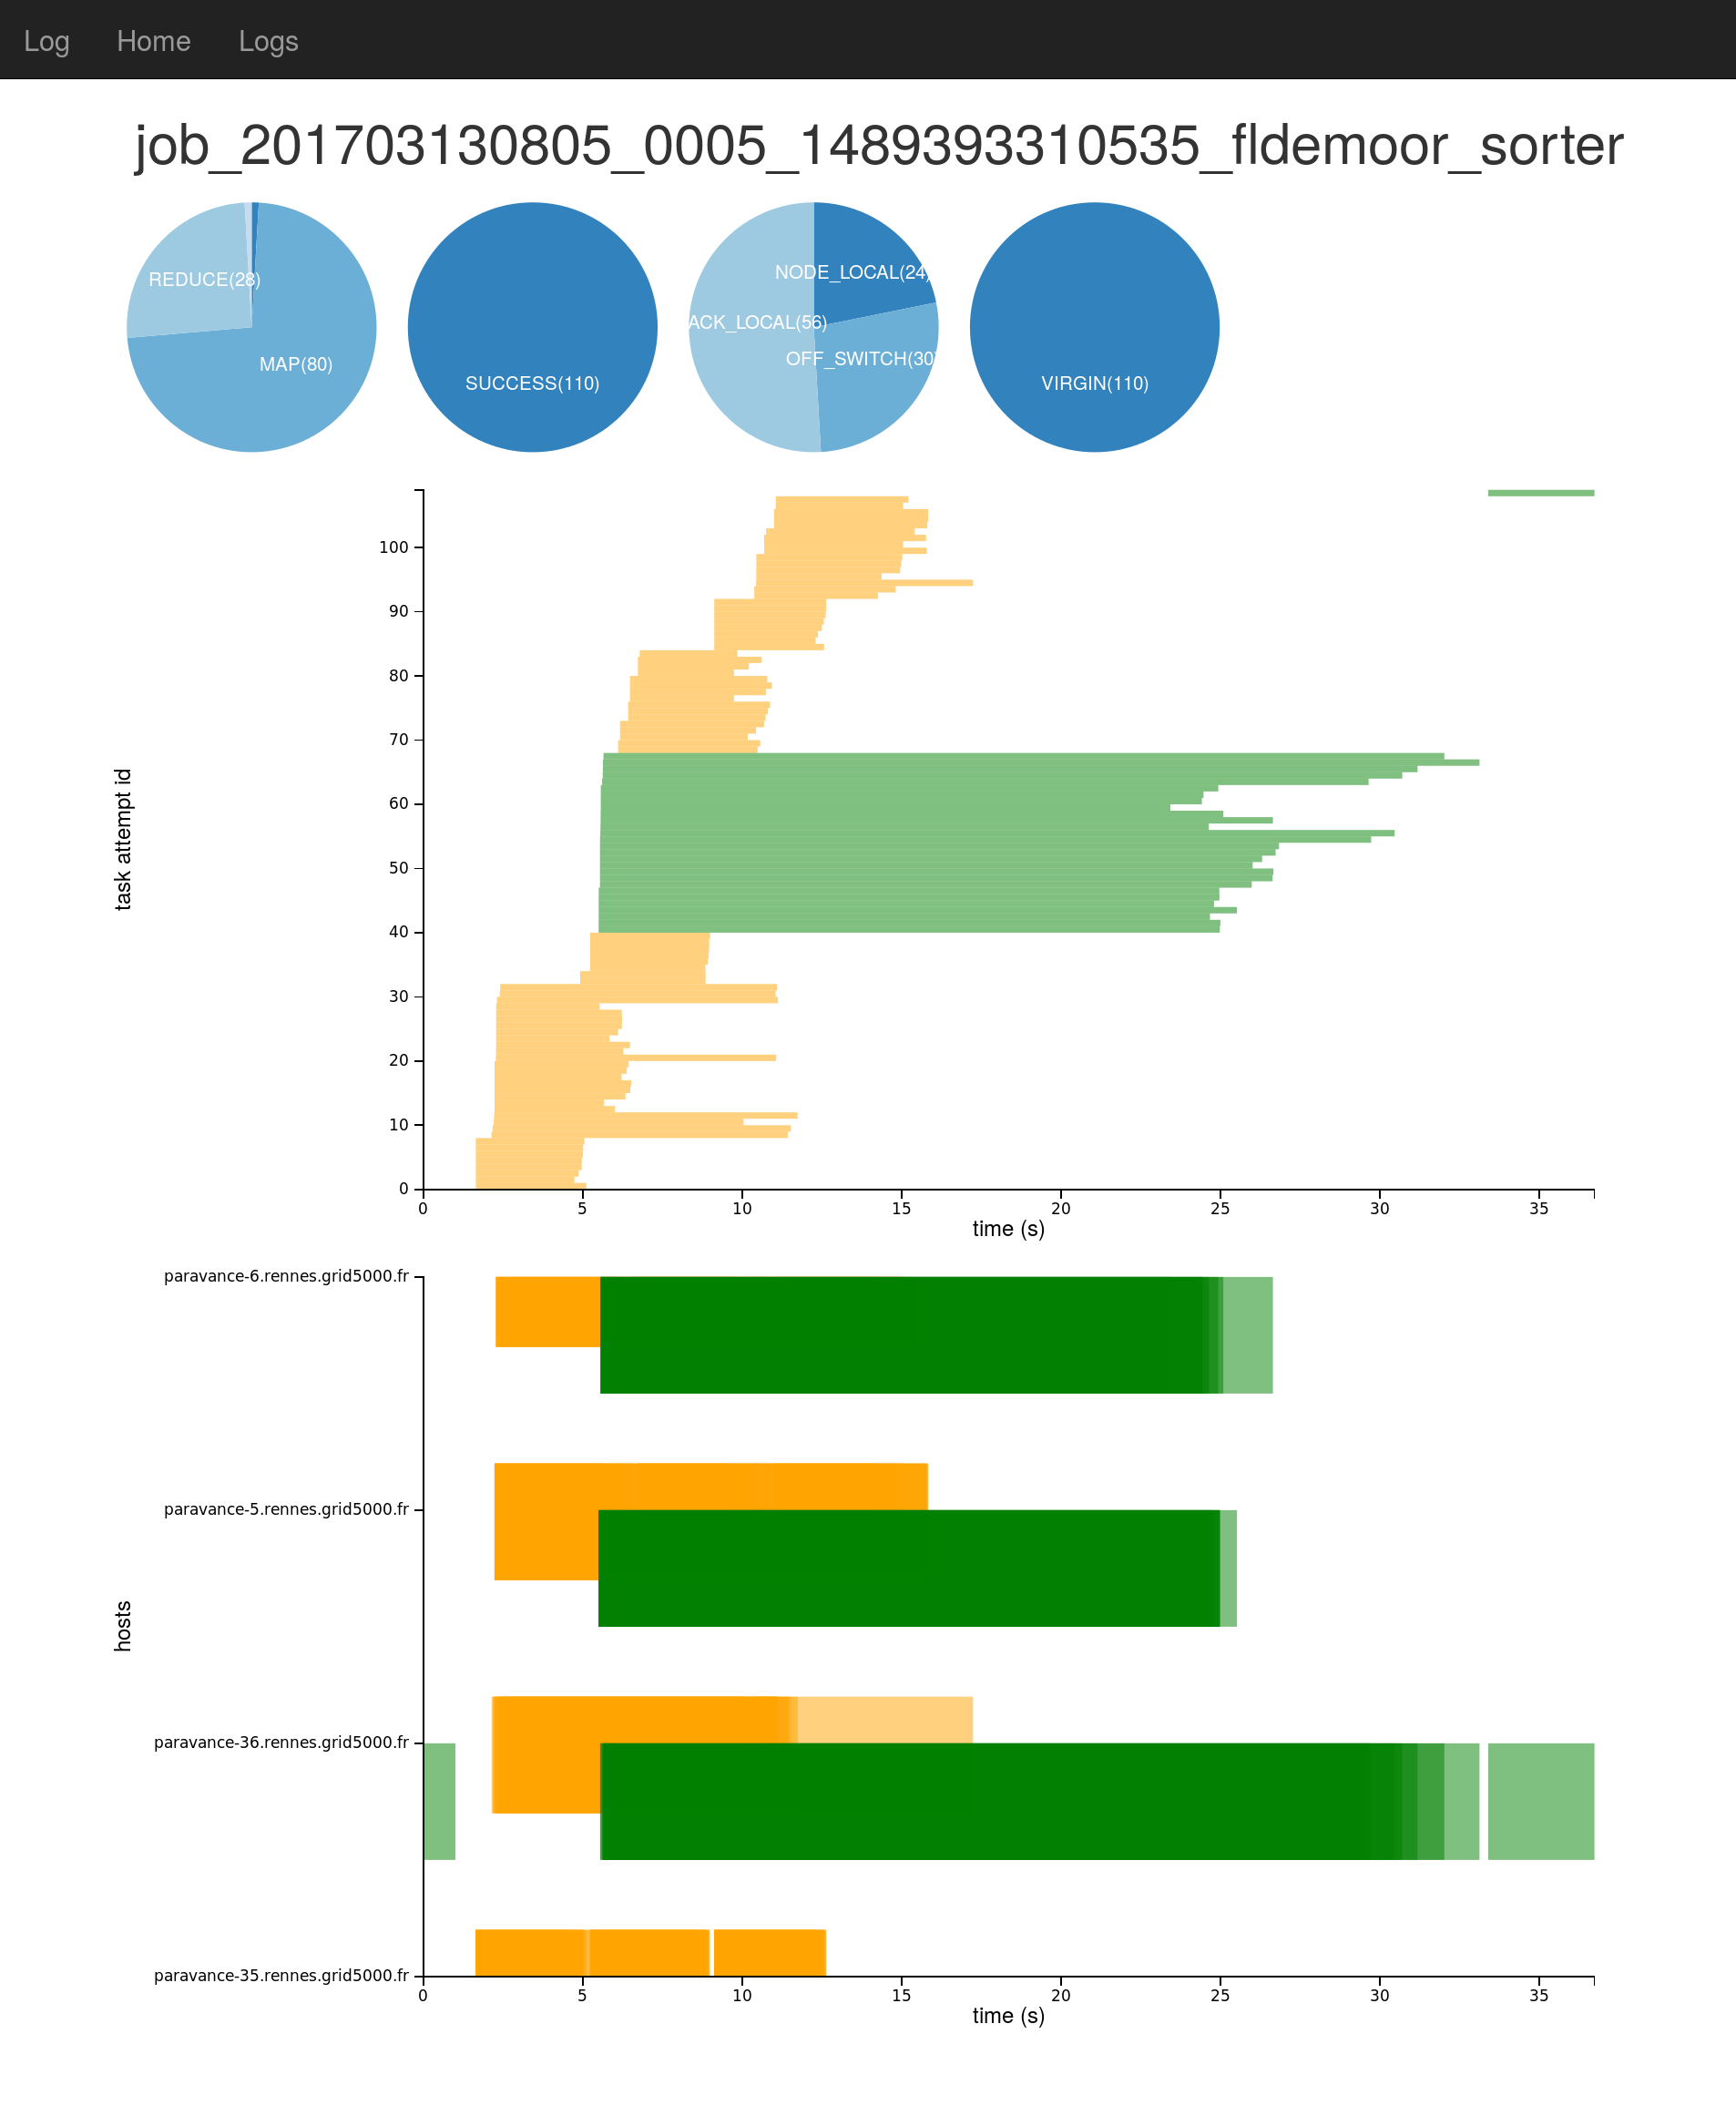
\includegraphics[trim={3.5cm 3.5cm 3.5cm 3.5cm},clip,width=\textwidth]{job_201703130805_0005_1489393310535_fldemoor_sorter_attempts.png}
    \caption{Question 1.1: Without speculation, with stress}
    \label{1.1.specOff.Stress}
\end{figure}
\newpage

\begin{figure}[!ht]
    \centering
    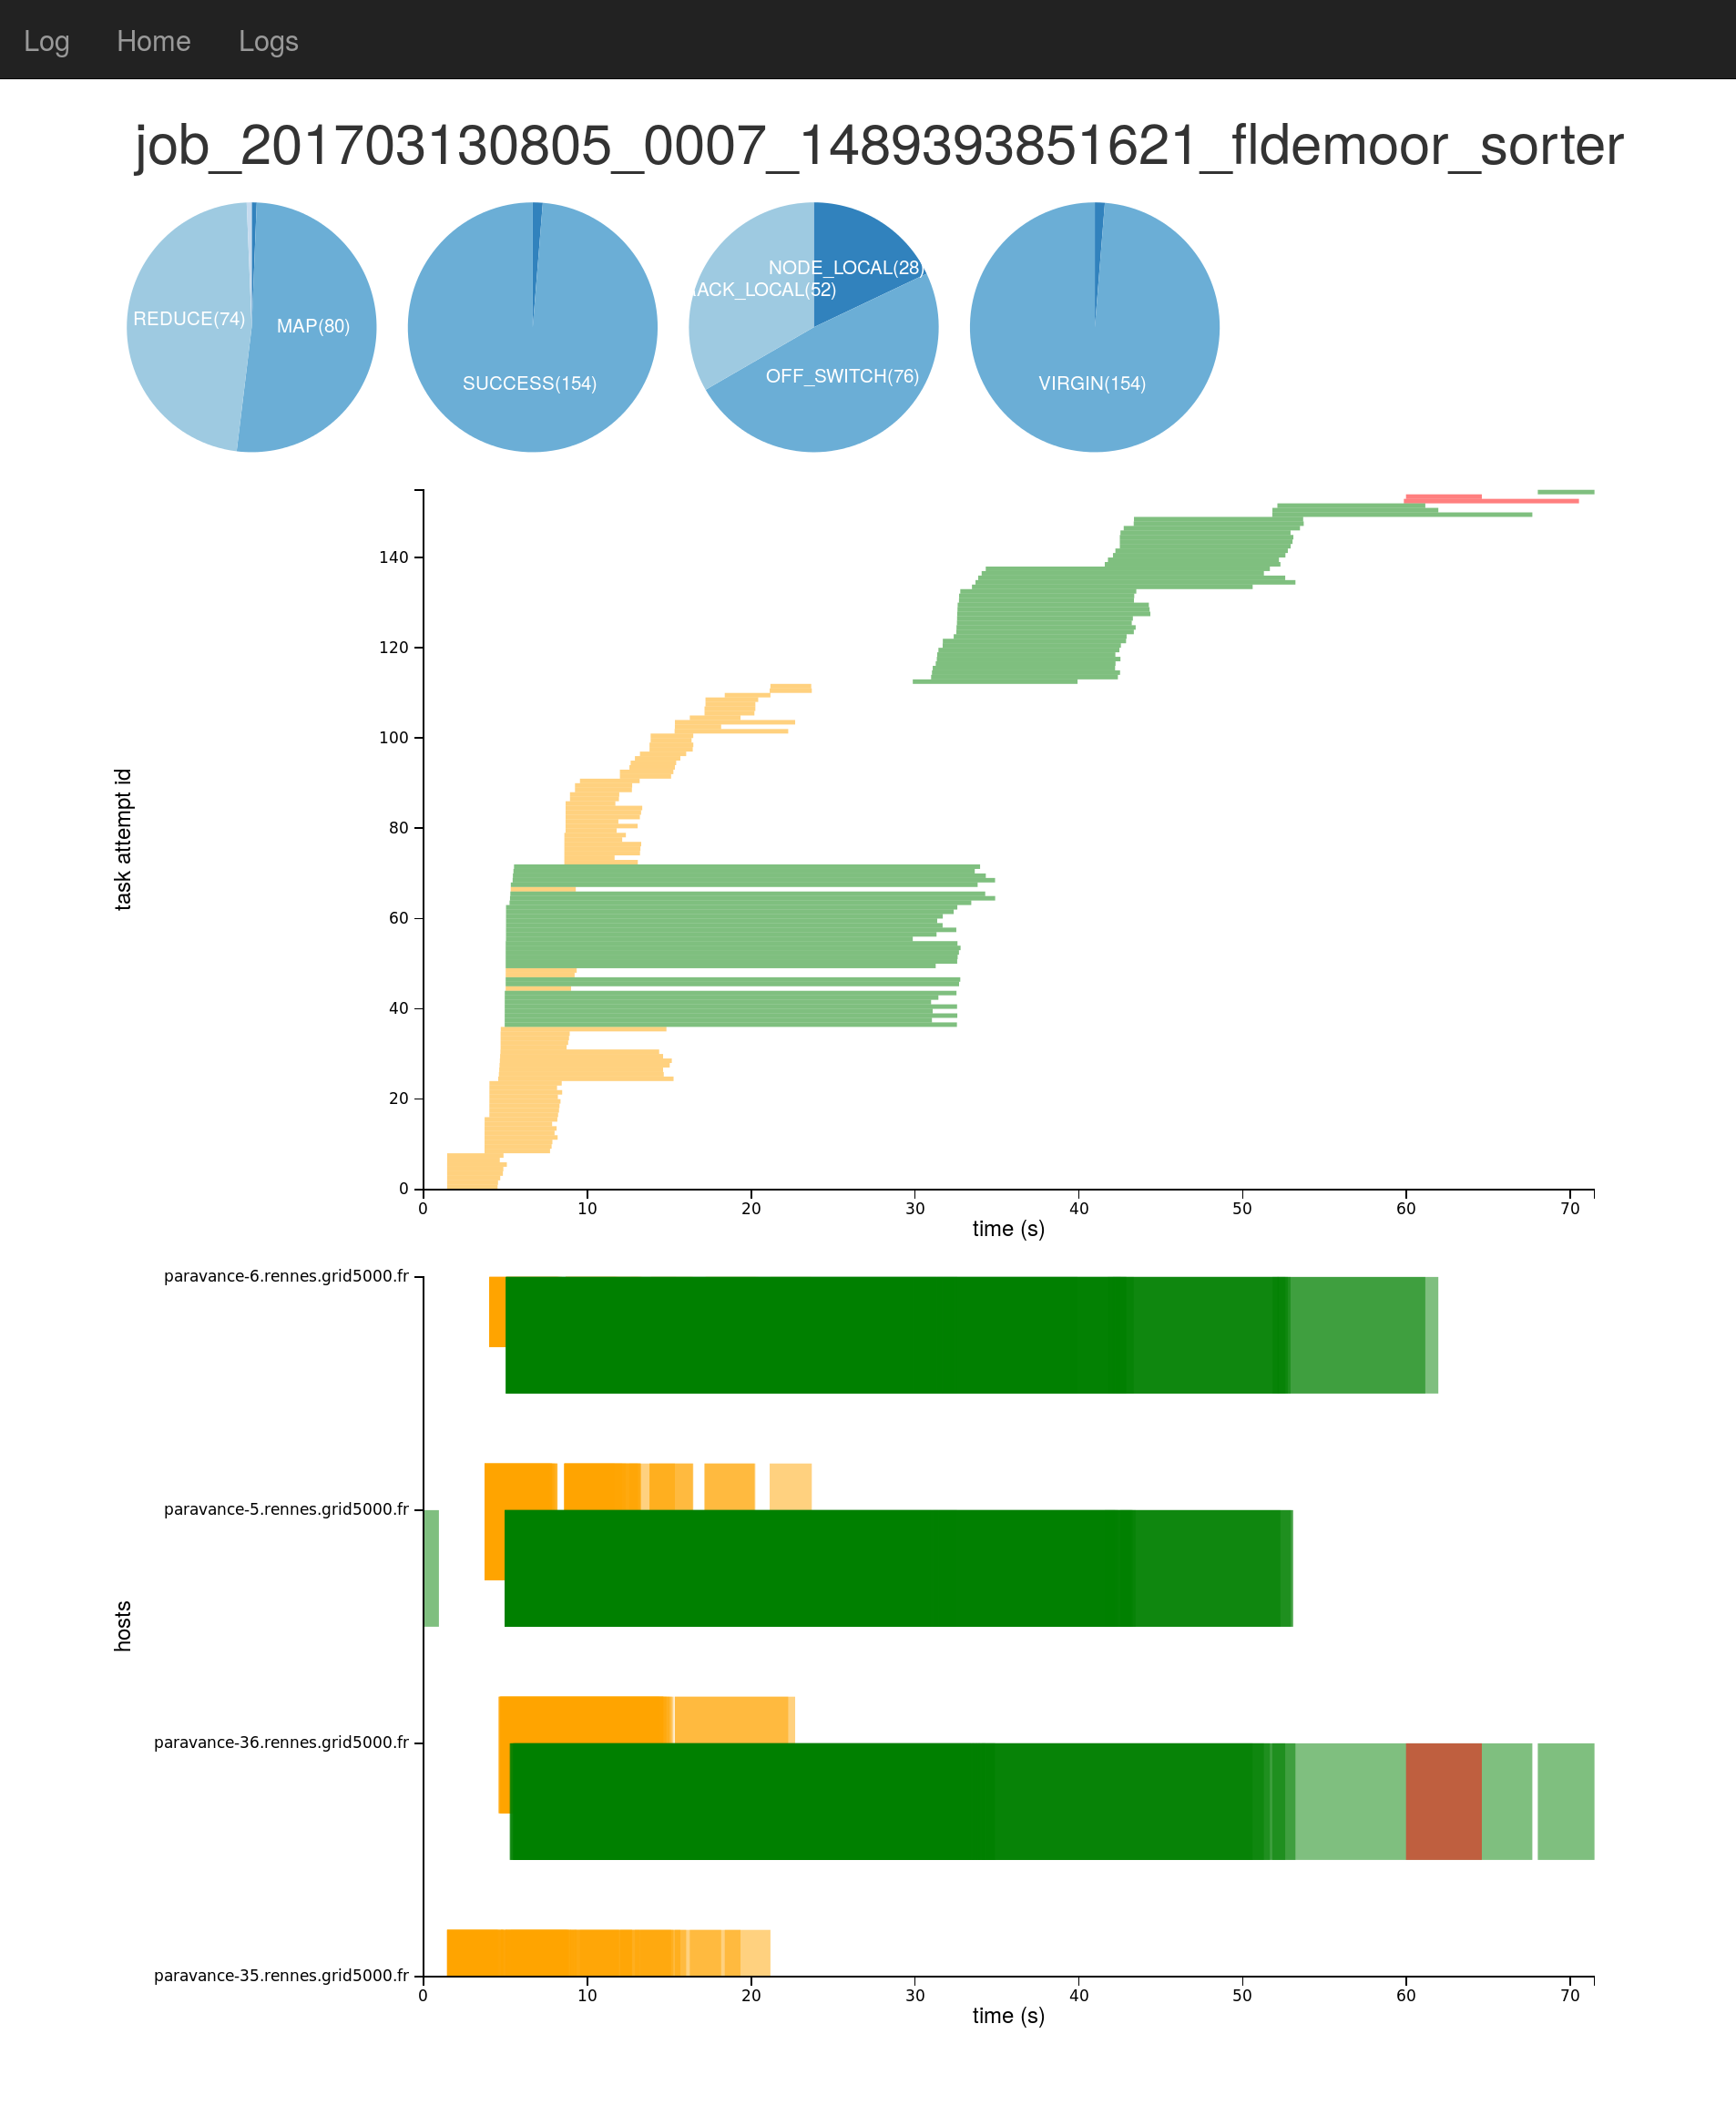
\includegraphics[trim={3.5cm 3.5cm 3.5cm 3.5cm},clip,width=\textwidth]{job_201703130805_0007_1489393851621_fldemoor_sorter_attempts.png}
    \caption{Question 1.1: With speculation, with stress}
    \label{1.1.specOn.Stress}
\end{figure}
\newpage

\section{Question 1.2}

\begin{figure}[!ht]
    \centering
    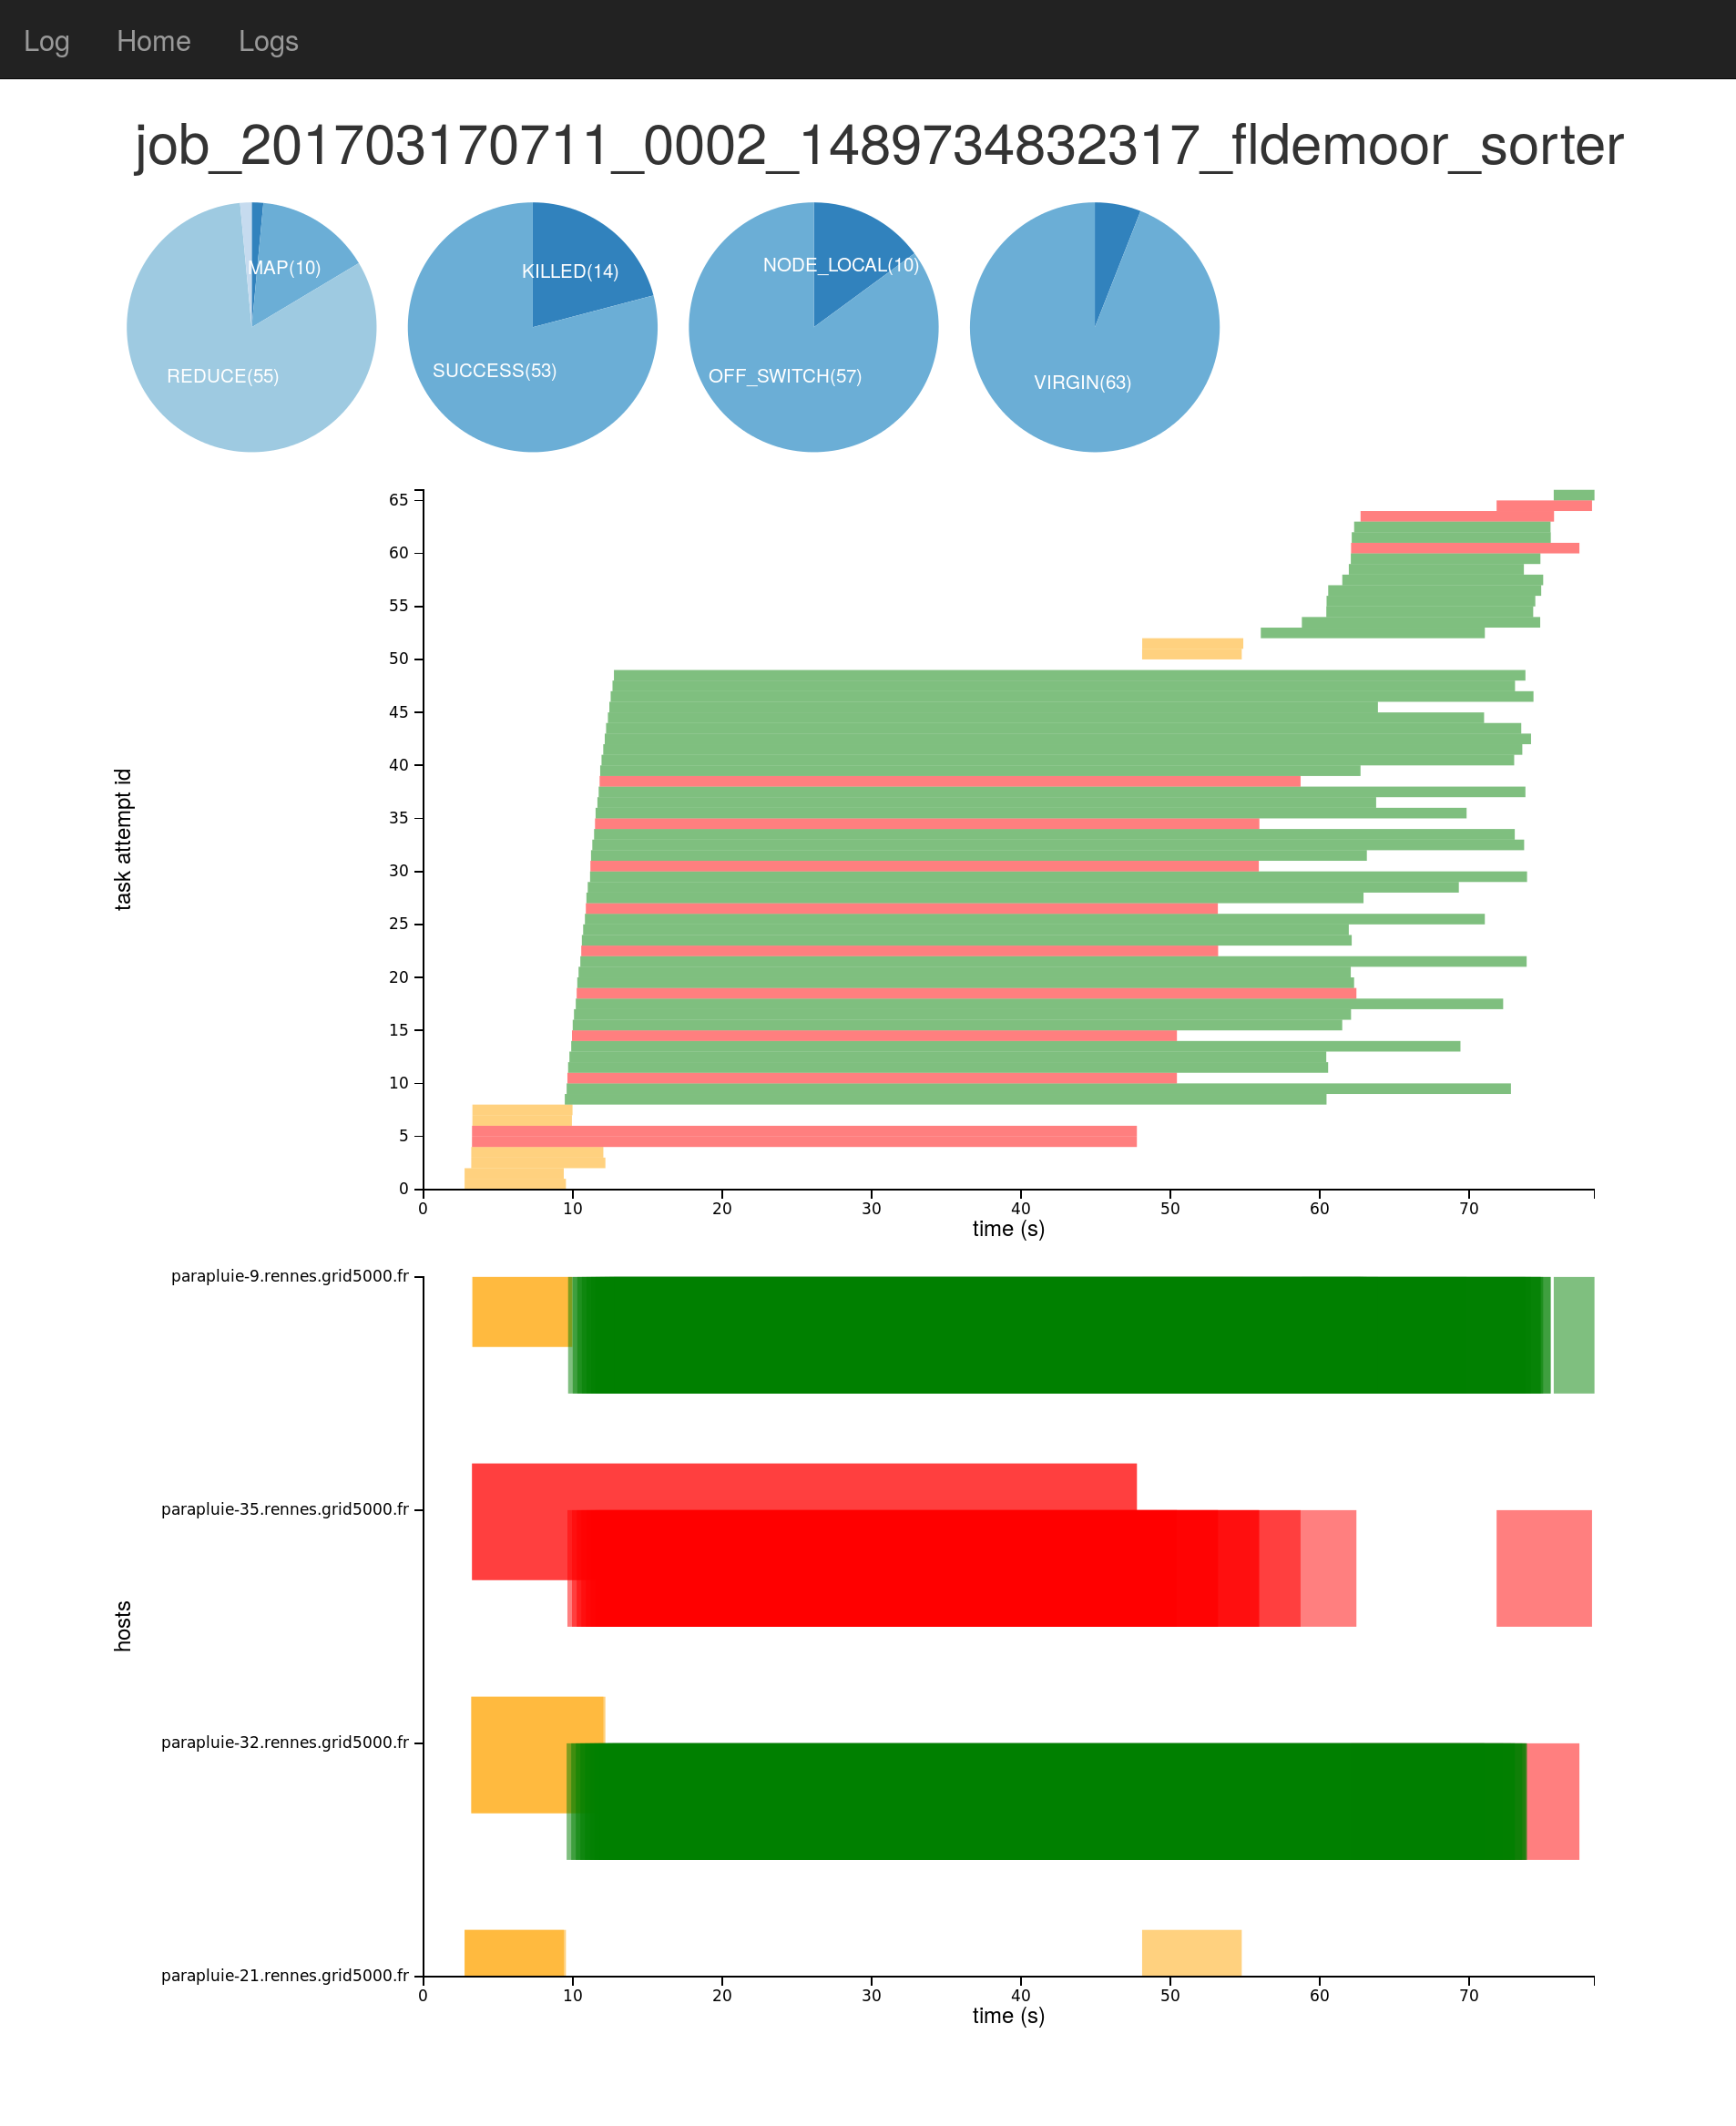
\includegraphics[width=\textwidth]{job_201703170711_0002_1489734832317_fldemoor_sorter_attempts.png}
    \caption{Question 1.2: Expiry 30 seconds, kill after map tasks completion}
    \label{1.2.30s.reduce}
\end{figure}
\newpage

\begin{figure}[!ht]
    \centering
    \includegraphics[width=\textwidth]
    \caption{Question 1.2: Expiry 60 seconds, kill after map tasks completion}
    \label{1.2.60s.reduce}
\end{figure}
\newpage

\section{Question 2.1}

\begin{figure}[!ht]
    \centering
    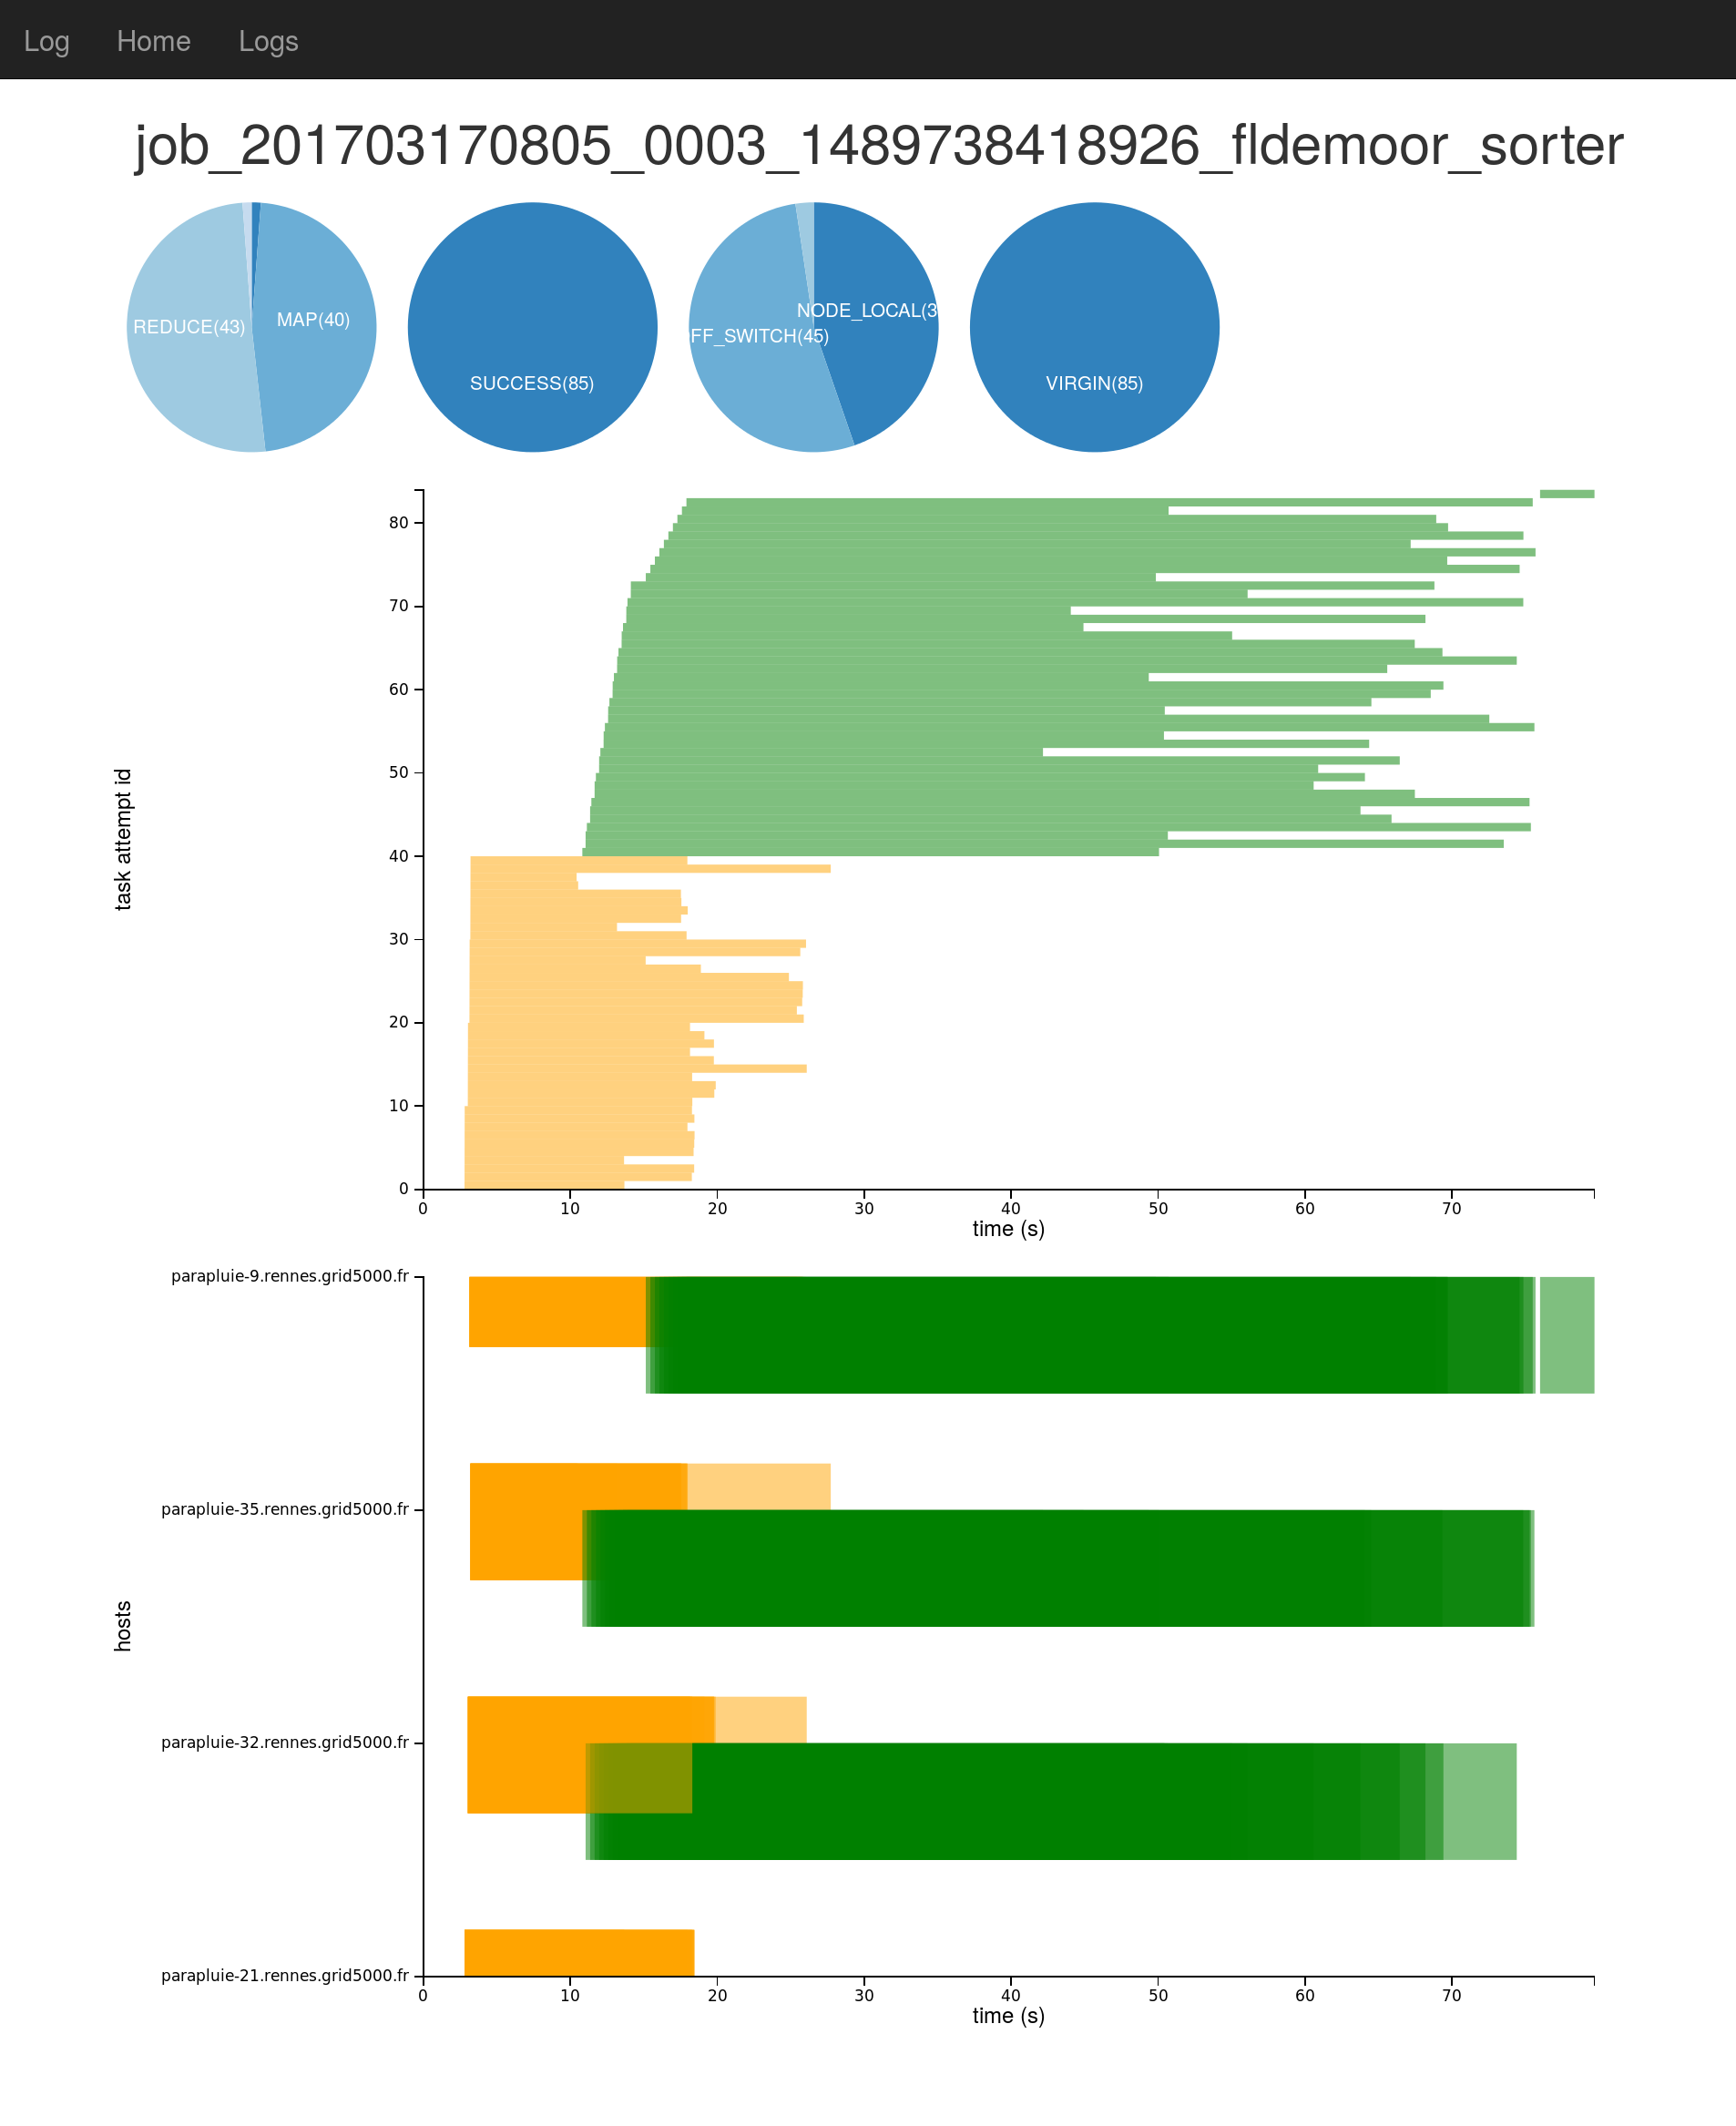
\includegraphics[width=\textwidth]{job_201703170805_0003_1489738418926_fldemoor_sorter_attempts.png}
    \caption{Question 2.1: Sort benchmark, 5\% slow-start}
    \label{2.1.sort.5}
\end{figure}
\newpage

\begin{figure}[!ht]
    \centering
    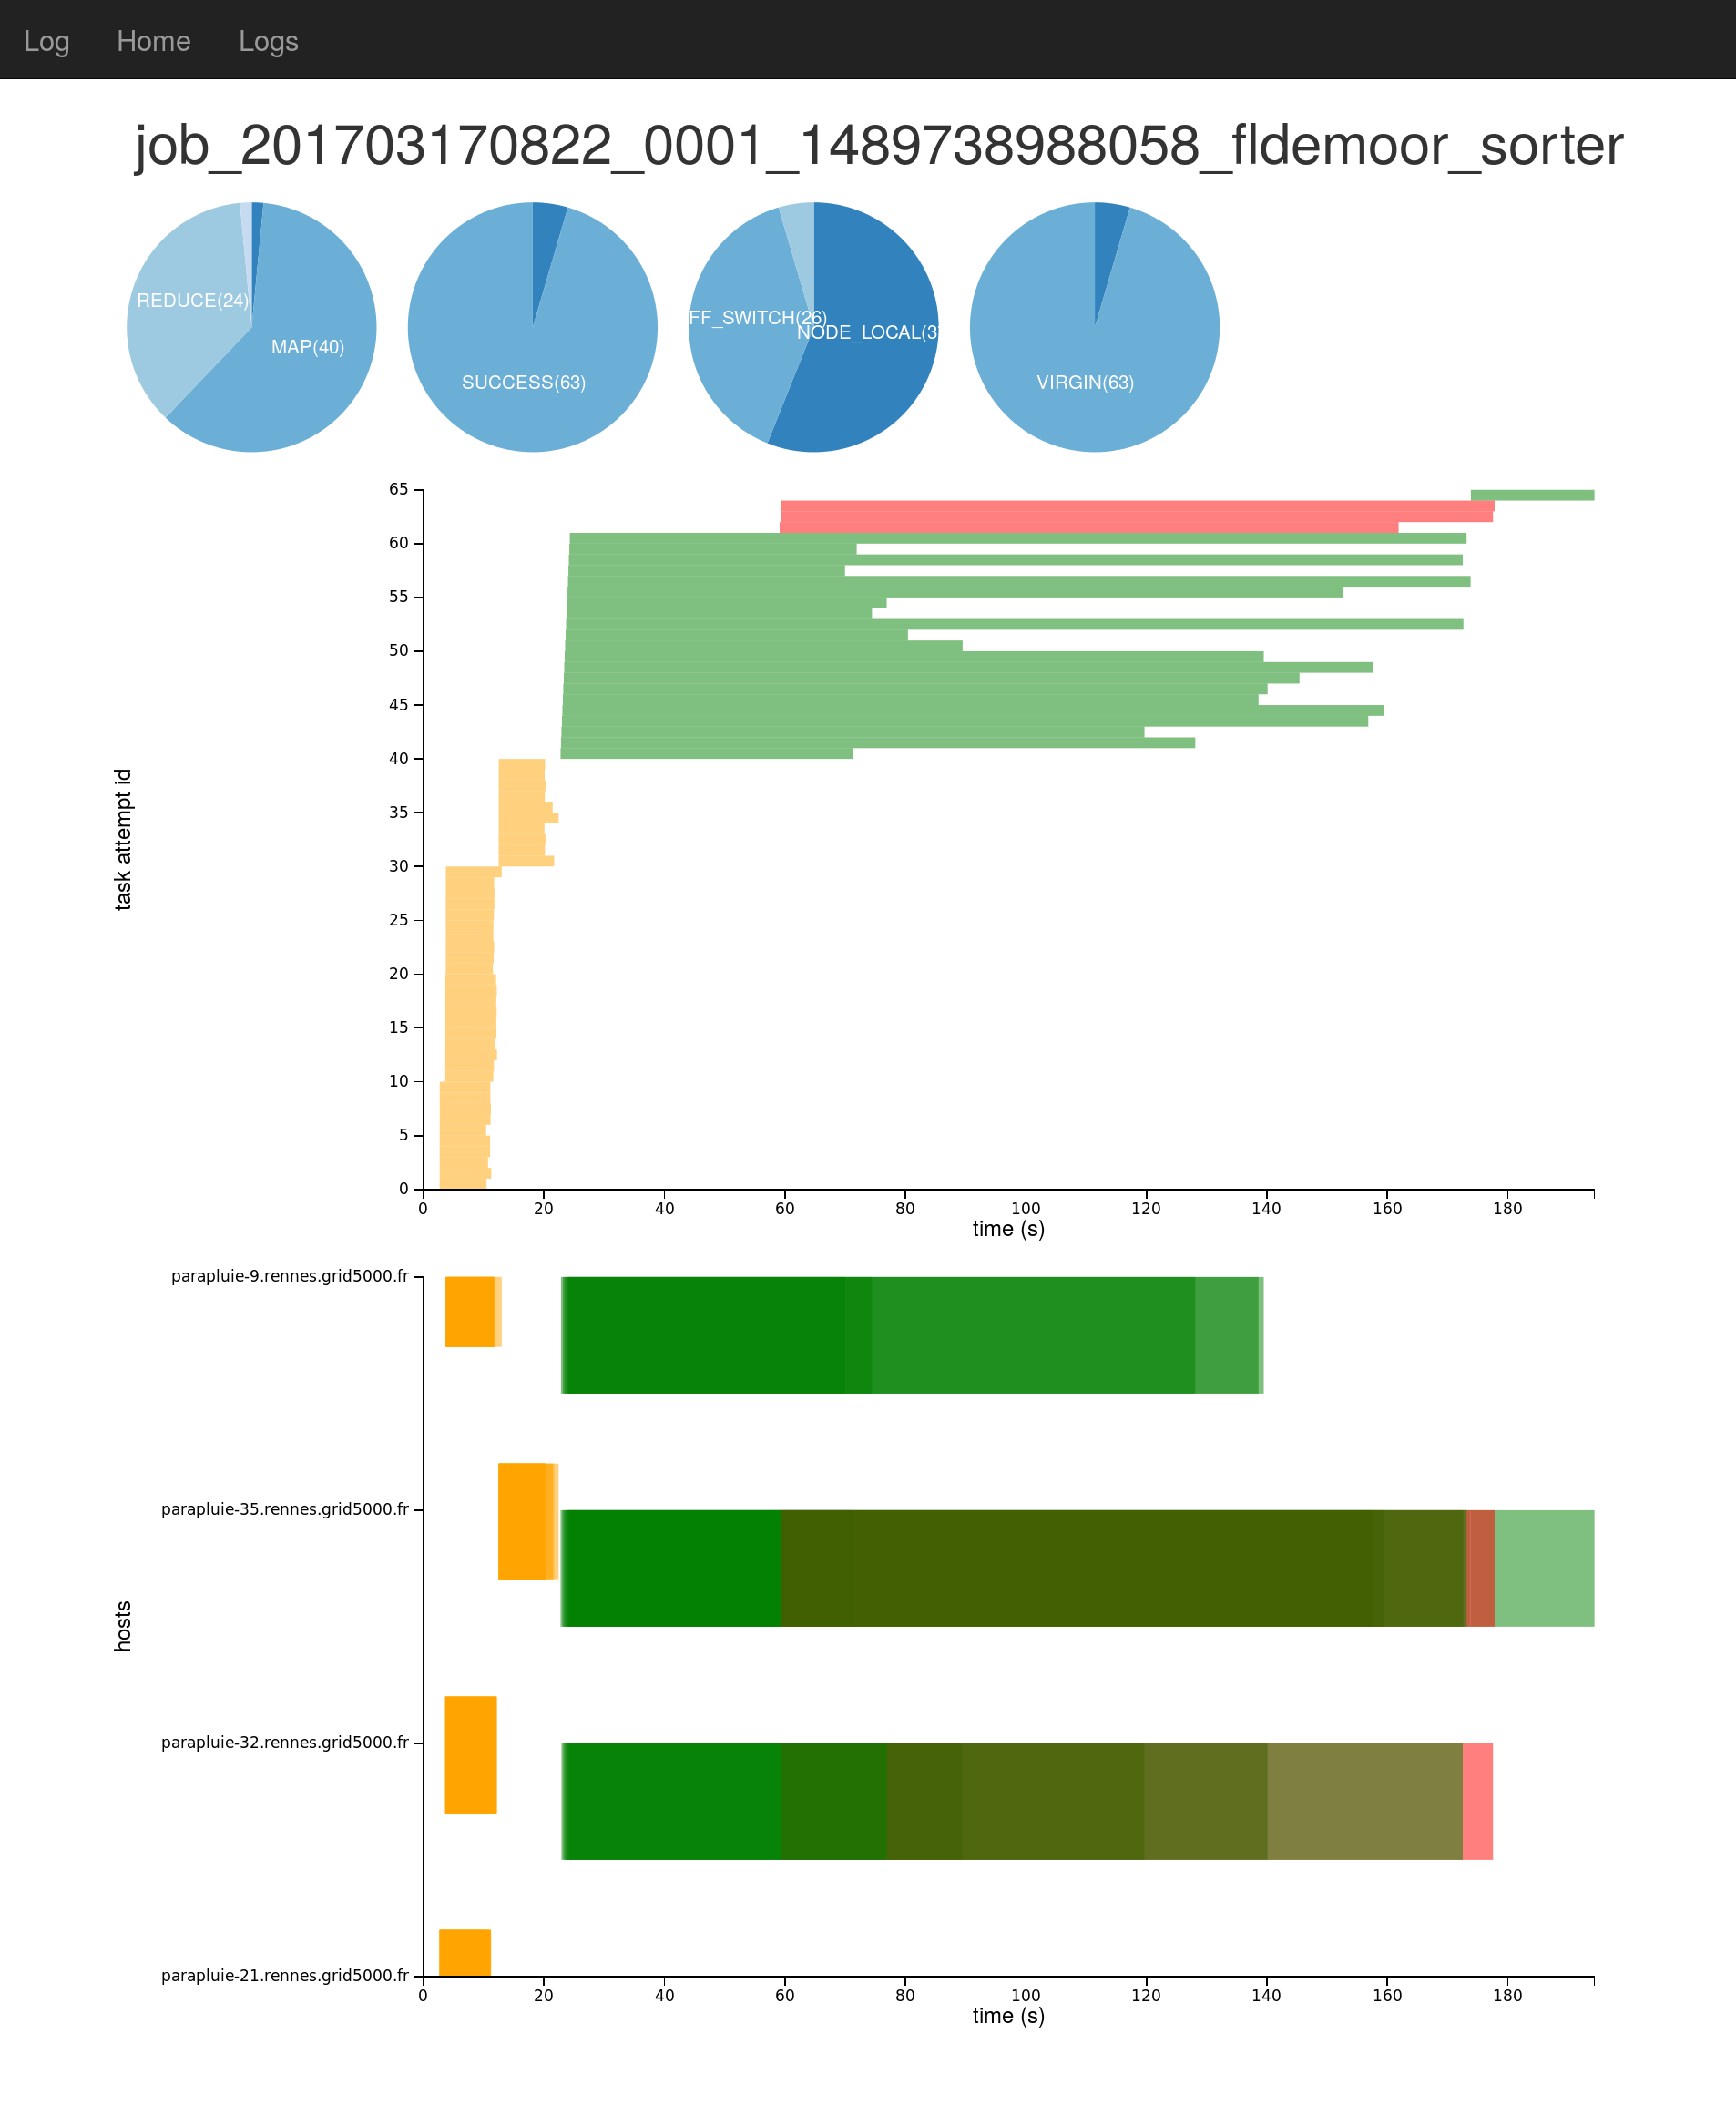
\includegraphics[width=\textwidth]{job_201703170822_0001_1489738988058_fldemoor_sorter_attemps.png}
    \caption{Question 2.1: Sort benchmark, 100\% slow-start}
    \label{2.1.sort.100}
\end{figure}
\newpage

\begin{figure}[!ht]
    \centering
    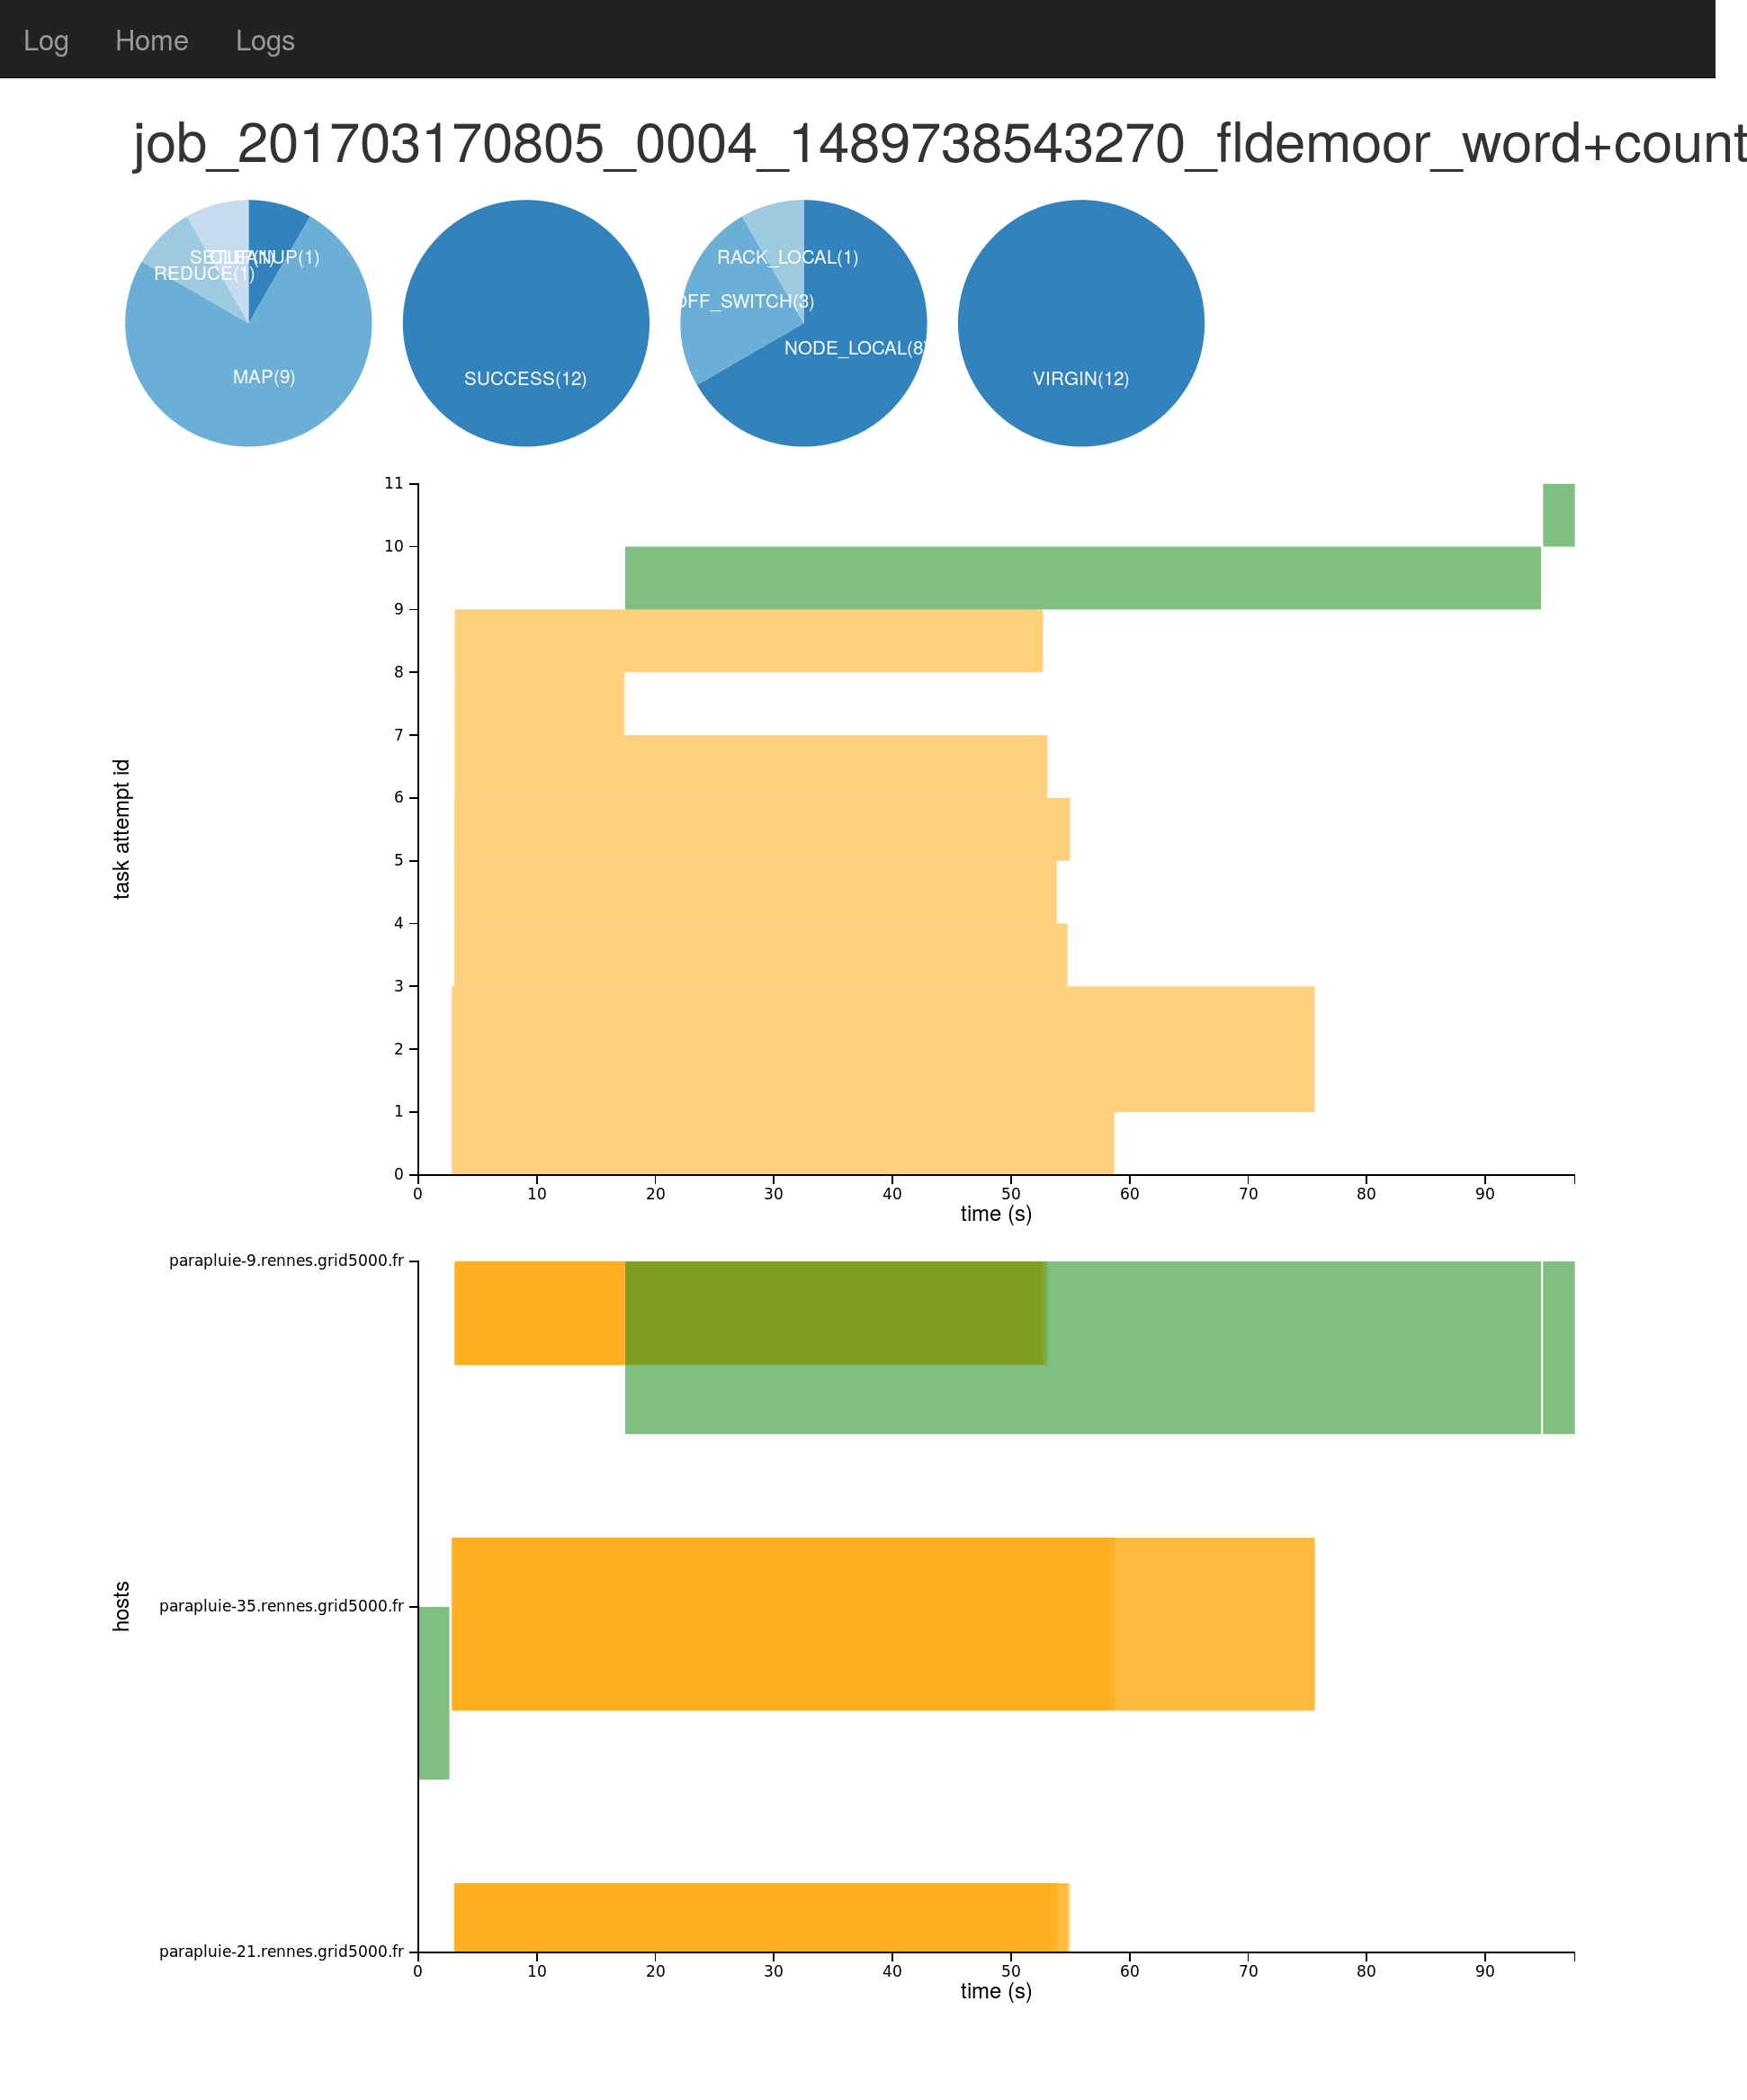
\includegraphics[width=\textwidth]{job_201703170805_0004_1489738543270_fldemoor_word+count_attempts.png}
    \caption{Question 2.1: Word count benchmark, 5\% slow-start}
    \label{2.1.wc.5}
\end{figure}
\newpage

\begin{figure}[!ht]
    \centering
    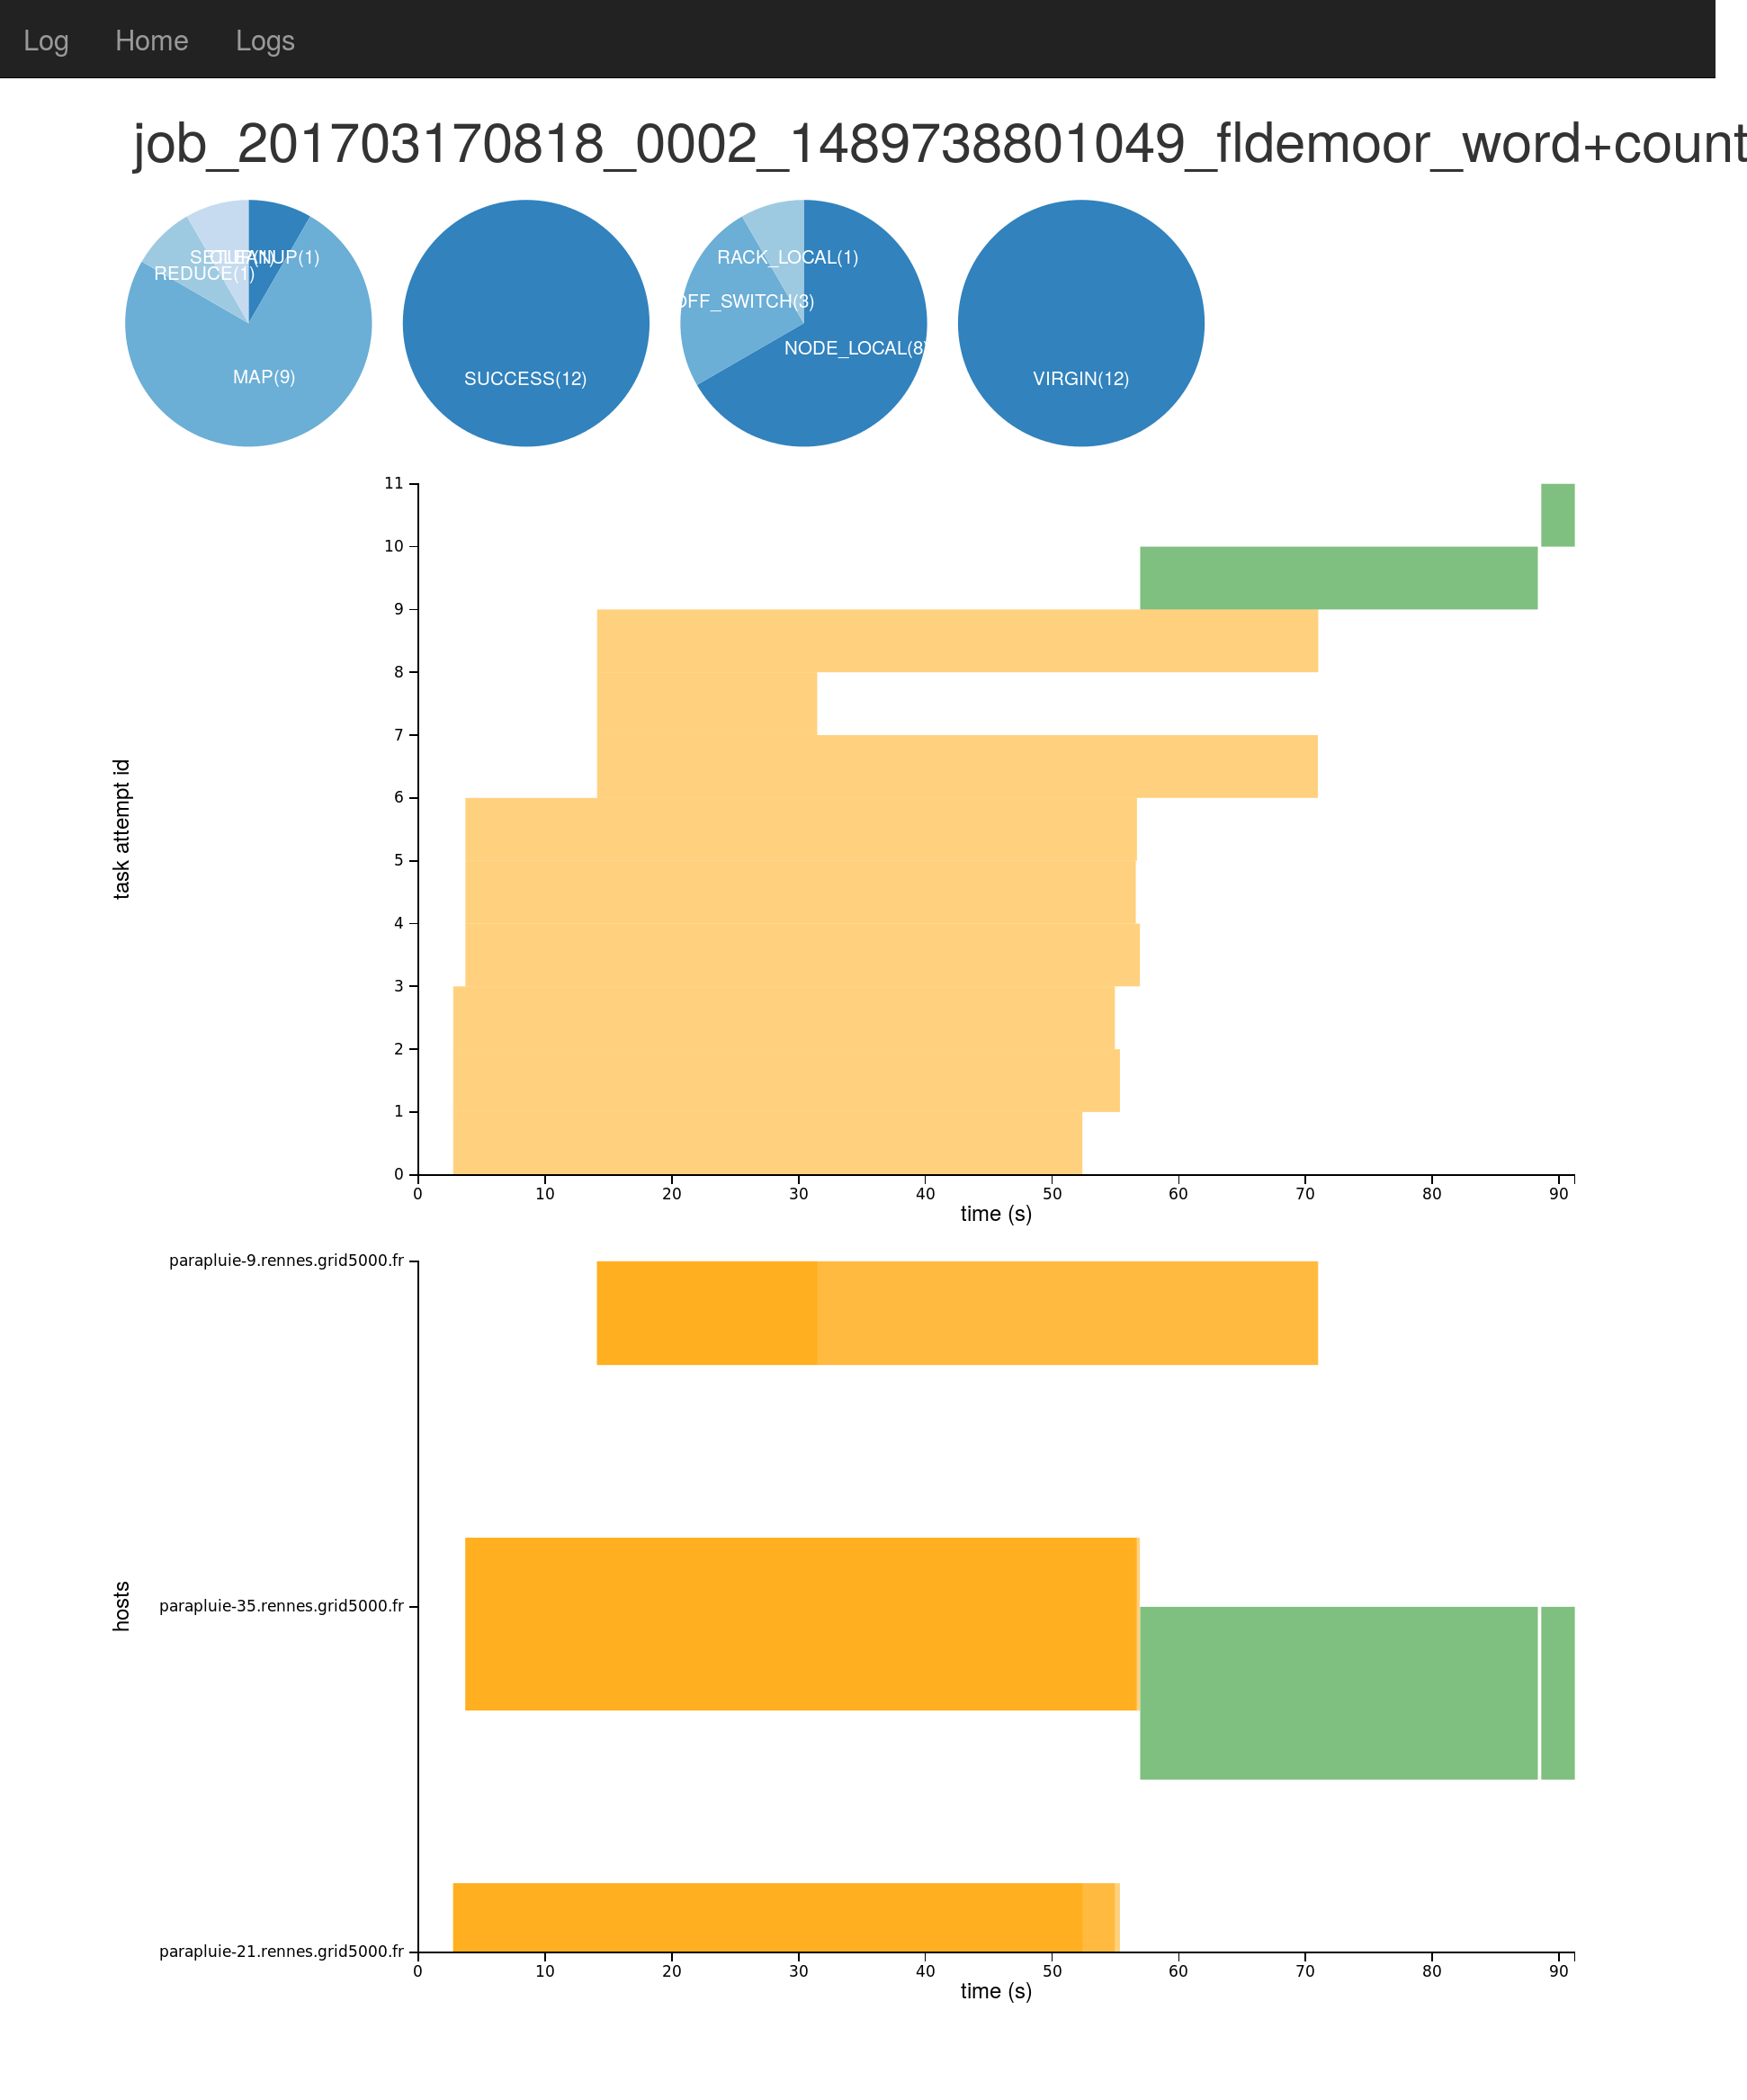
\includegraphics[width=\textwidth]{job_201703170818_0002_1489738801049_fldemoor_word+count_attemps.png}
    \caption{Question 2.1: Word count benchmark, 50\% slow-start}
    \label{2.1.wc.50}
\end{figure}
\newpage

\begin{figure}[!ht]
    \centering
    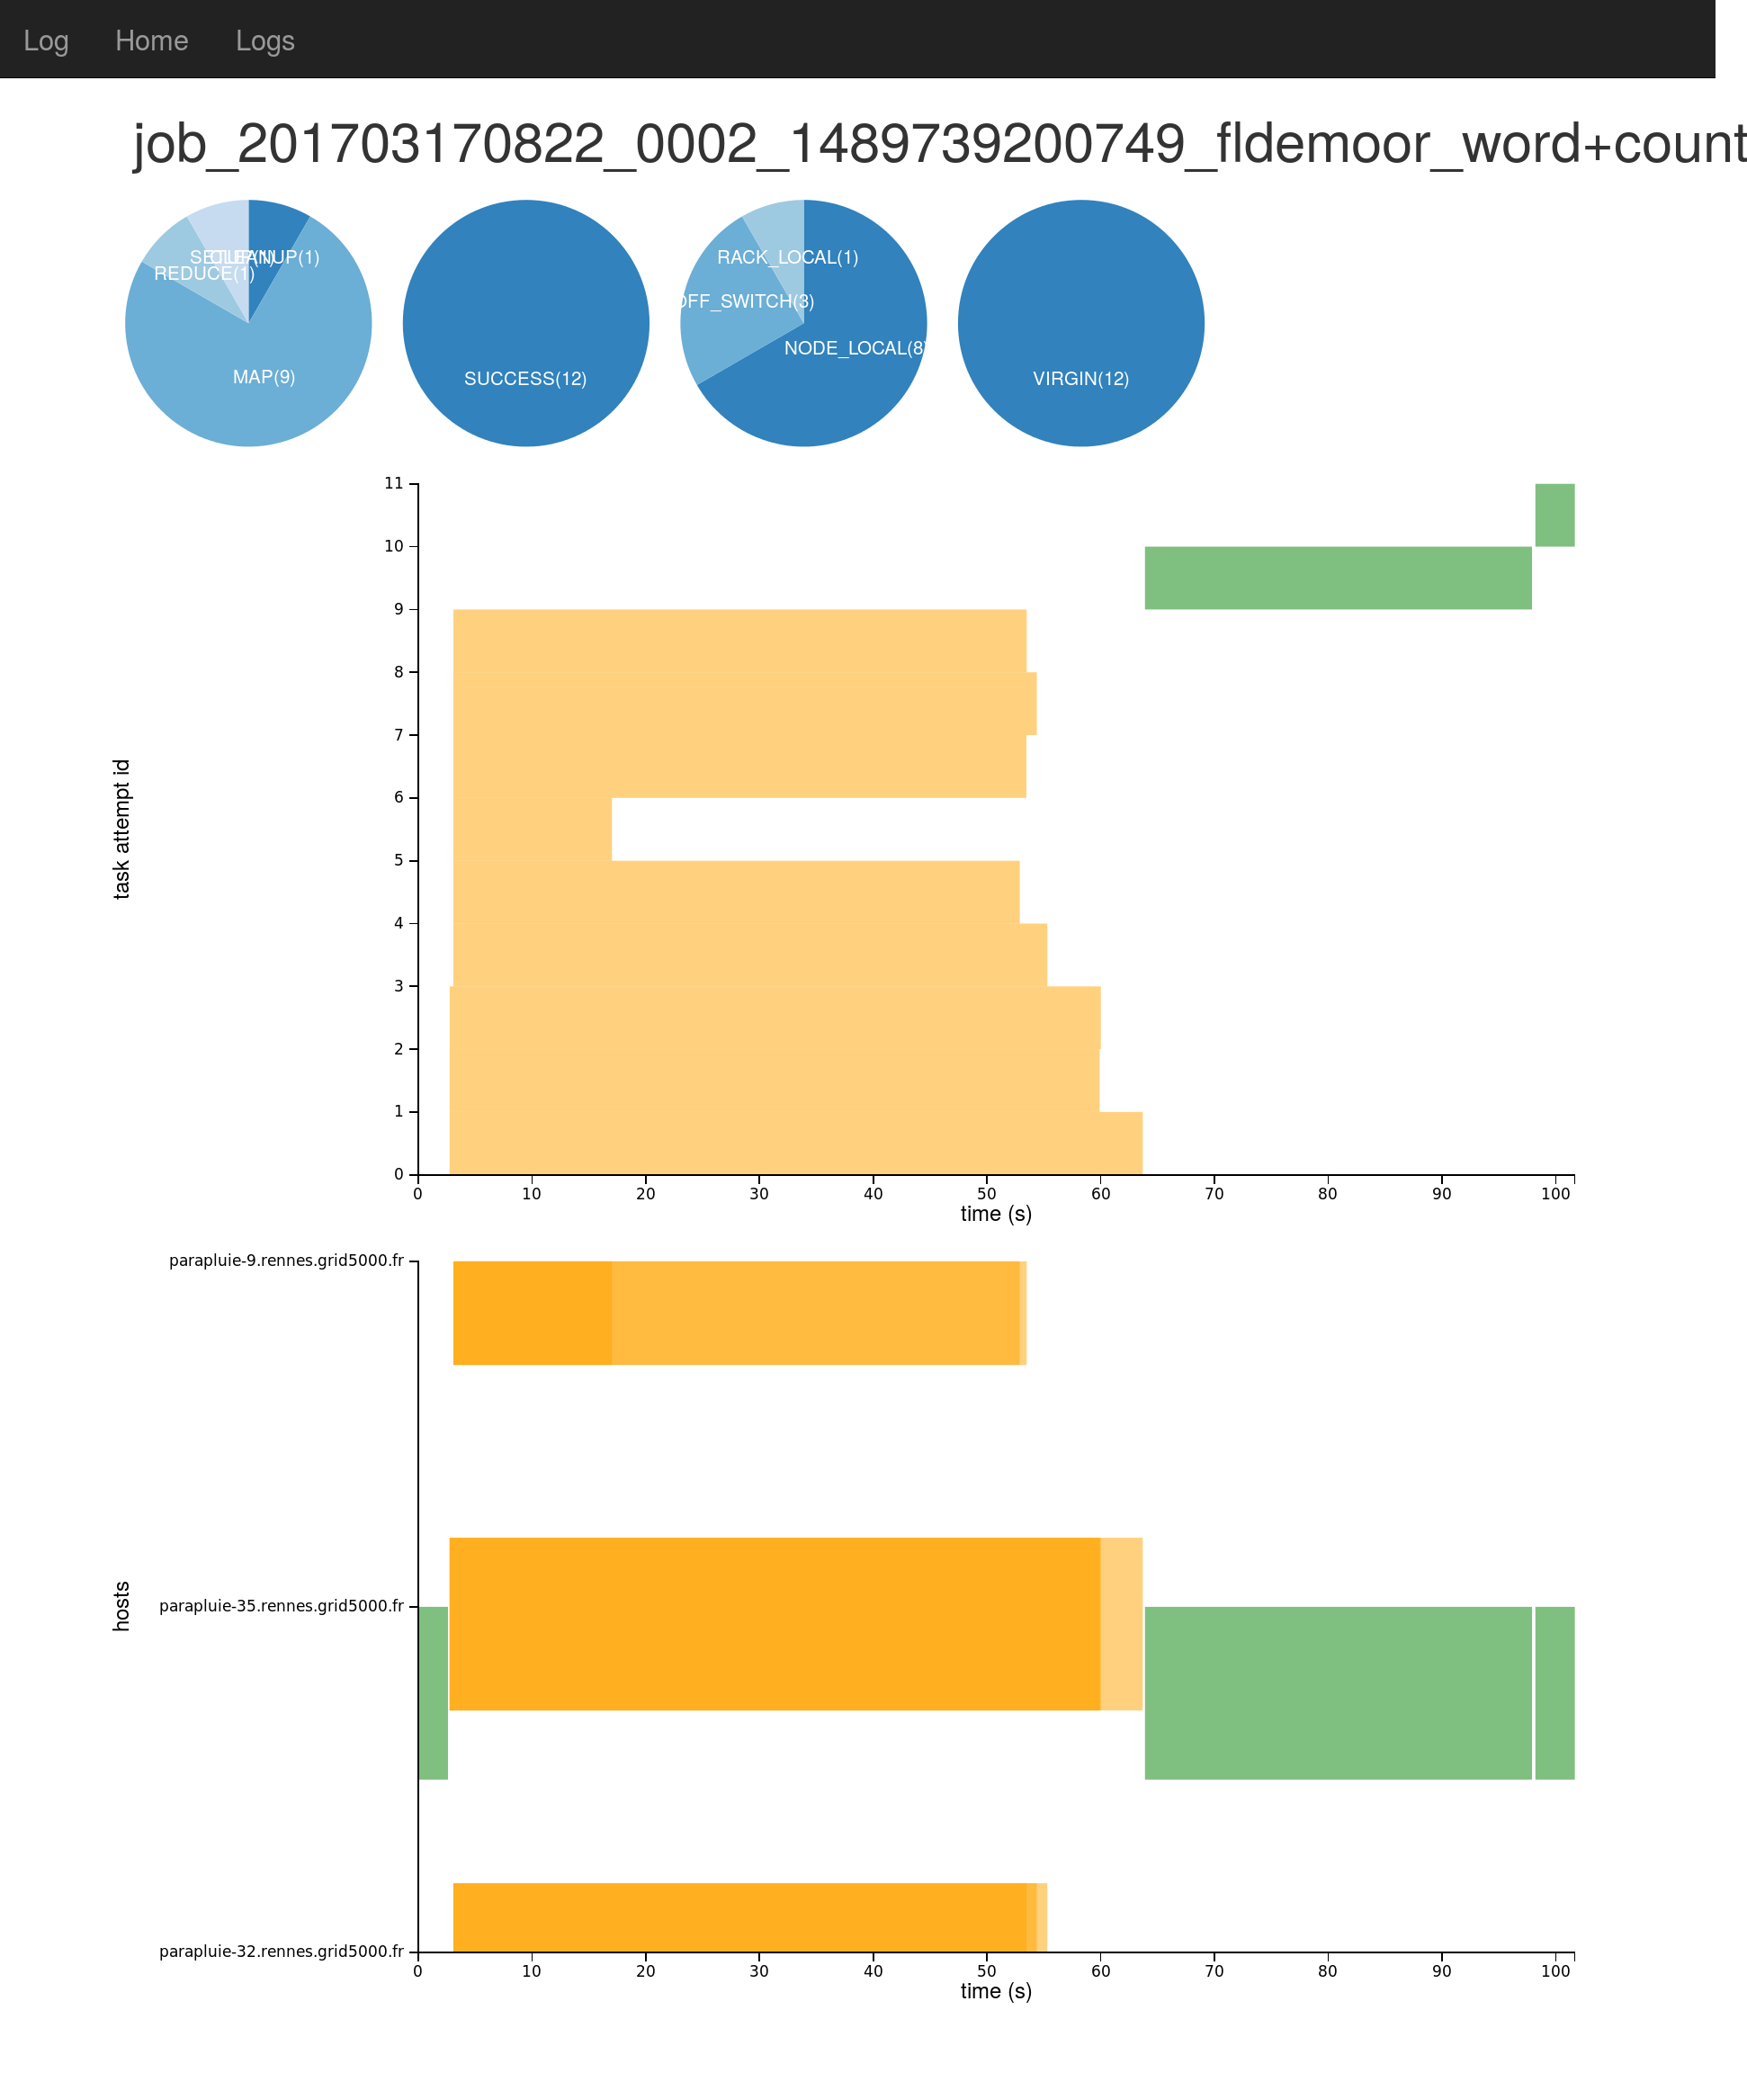
\includegraphics[width=\textwidth]{job_201703170822_0002_1489739200749_fldemoor_word+count_attempts.png}
    \caption{Question 2.1: Word count benchmark, 100\% slow-start}
    \label{2.1.wc.100}
\end{figure}
\newpage



\end{document}
